\documentclass[11pt]{article}
\usepackage[scaled=0.92]{helvet}
\usepackage{geometry}
\geometry{letterpaper,tmargin=1in,bmargin=1in,lmargin=1in,rmargin=1in}
\usepackage[parfill]{parskip} % Activate to begin paragraphs with an empty line rather than an indent %\usepackage{graphicx}
\usepackage{amsmath,amssymb, mathrsfs, dsfont, stackrel}
\usepackage{tabularx}
\usepackage[font=footnotesize,labelfont=bf]{caption}
\usepackage{graphicx}
\usepackage{xcolor}
%\usepackage[linkbordercolor ={1 1 1} ]{hyperref}
%\usepackage[sf]{titlesec}
\usepackage{natbib}
\usepackage{../../Tianpei_Report}
%\usepackage{appendix}
%\usepackage{algorithm}
%\usepackage{algorithmic}

%\renewcommand{\algorithmicrequire}{\textbf{Input:}}
%\renewcommand{\algorithmicensure}{\textbf{Output:}}



\begin{document}
\title{Summary of Monte Carlo Sampling Methods}
\author{Tianpei Xie}
\date{Sep. 28th., 2022 }
\maketitle
\tableofcontents
\newpage
\allowdisplaybreaks
\section{Basic Concepts}
\subsection{Random variable generation}
\begin{itemize}
\item The most fundamental methods for random variable generation is the \emph{\textbf{uniform pseudo-random number generator}}.
\begin{definition}
 A \emph{uniform pseudo-random number generator} is an algorithm which, starting from an initial value $u_0$ and a transformation $D$, produces a sequence $(u_i) = (D^i(u_{0}))$ of values in $[0, 1]$. For all $n$, the values $(u_1, \ldots , u_n)$ reproduce the behavior of an \emph{iid} sample $(V_1, \ldots, V_n)$ of uniform random variables when compared through a usual set of tests.
 \end{definition}

\item Given uniform distribution $\cU[0,1]$, and a known c.d.f. $F(x)$, we can generate samples via the \emph{\textbf{inverse transform}} method. \citep{robert1999monte}

\begin{definition}
For a \textbf{\emph{non-decreasing}} function $F$ on $\bR$, the \underline{\emph{\textbf{generalized inverse}}} of $F$, $F^{-}$, is the function defined by
\begin{align}
F^{-}(u) &= \inf\{x \in \cR(F): F(x) \ge u \}. \label{eqn: quantile_function}
\end{align} where $\cR(F)$ is the range of $F$. If $F$ is the cumulative distribution function $F_{X}(x) = P(X \le x)$, then $F_{X}^{-1}$ is called \underline{\textbf{\emph{quantile function}}}.
\end{definition}

\item We then have the following lemma, sometimes known as the \textbf{probability integral transform}, which gives us a representation of any random variable as a transform of a uniform random variable.
\begin{lemma} \citep{robert1999monte}\\
If $U \sim \cU[0,1]$, then the random variable $F^{-}(U)$ has the distribution $F$.
\end{lemma}

\item Theoretically, any random variable can be generated using the inverse transform. But in practice, it is only available when we can compute the c.d.f and its inverse $F^{-}$ explicitly. 
\end{itemize}

\subsection{Why Monte Carlo ?}
\begin{itemize}
\item The most fundamental operations in probabilistic modeling and statistics involve \underline{\emph{\textbf{integration}}} on \underline{\textbf{high dimensional spaces}}. For example, 
\begin{itemize}
\item \underline{\emph{\textbf{Expectation}}}: 
\begin{align}
\E{\mb{X}\sim p}{h(\mb{X})} &= \int_{\cX}h(\mb{x})p(\mb{x}) d\mb{x}  \label{eqn: exp_integration}
\end{align} where $\mb{x}:= [x_1,\ldots, x_d]$

\item \underline{\emph{\textbf{Marginalization}}}:
\begin{align*}
P(x_1,\ldots, x_{i-1}, x_{i+1} \ldots, x_d) &= \int_{x_i \in \cX_i}P(x_1,\ldots, x_{i-1}, x_i, x_{i+1} \ldots, x_d) d x_i
\end{align*}

\item \underline{\emph{\textbf{Conditioning}}}:
\begin{align*}
P(x_1,\ldots, x_{i-1}, x_{i+1} \ldots, x_d \,|\, X_i = x_i) 
&= \frac{P(x_1,\ldots, x_{i-1}, x_i, x_{i+1} \ldots, x_d)}{ \int_{\mb{x}_{-i} \in \mb{X}_{-i}}P(x_1,\ldots, x_{i-1}, x_i, x_{i+1} \ldots, x_d) d\mb{x}_{-i}}
\end{align*} where $\mb{x}_{-i} = [x_1,\ldots, x_{i-1}, x_{i+1} \ldots, x_d]$.
\end{itemize}

\item In \emph{\textbf{Bayesian inference}} and analysis, we need to compute \emph{posterior distribution} given data via \textbf{the Bayes rule}: 
\begin{align*}
P(\mb{\Theta} | \cD) &= \frac{P(\cD | \mb{\Theta}) P(\mb{\Theta})}{P(\cD)}\\
 &= \frac{P(\cD | \mb{\Theta}) P(\mb{\Theta})}{\int_{\mb{\Theta}} P(\cD | \mb{\Theta}) P(\mb{\Theta}) d \mb{\Theta}}\\
 \Rightarrow \log P(\mb{\Theta} | \cD)  &= \log P(\cD | \mb{\Theta}) + \log P(\mb{\Theta}) - \log \int_{\mb{\Theta}} P(\cD | \mb{\Theta}) P(\mb{\Theta}) d \mb{\Theta}
\end{align*} where $\cD: =\set{\mb{X}_1, \ldots, \mb{X}_n}$ are i.i.d. samples and $\mb{\Theta}$ is a set of parameters for model $p(\cD | \mb{\Theta})$.

The main challenge for Bayesian methods in high dimensional space is to compute the normalization factor and conditional expectation
\begin{align*}
Z &= \int_{\mb{\Theta}} P(\cD | \mb{\Theta}) P(\mb{\Theta}) d \mb{\Theta}. \\
\E{}{\mb{\Theta} | \cD} &= \int \mb{\Theta} P(\mb{\Theta} | \cD)  d\mb{\Theta}
\end{align*}

\item The \textbf{\emph{log-partition function}} in \textbf{exponential families} play a critical role since it defines a \emph{bijective mapping} from \emph{natural parameters} to \emph{mean parameters} and is related to \textbf{negative entropy} via \emph{variational principles}. The log-partition function for exponential families is a convex function as well.
\begin{align*}
A(\mb{\eta}) &= \log \int_{\Omega}\exp\paren{\inn{\mb{\eta}}{\mb{\phi}(\mb{x})}}d\mb{x}
\end{align*}

\item The \underline{\emph{\textbf{Monte Carlo methods}}} \emph{\textbf{approximate integration}} by the \emph{\textbf{empirical average}} over a set of samples $(\mb{X}_1, \ldots , \mb{X}_m)$ generated from the density $p$. Specifically from \eqref{eqn: exp_integration}, 
\begin{align}
\overline{h}_{m} &= \frac{1}{m}\sum_{i=1}^{m}h(\mb{X}_{i}) \label{eqn: exp_integration_monte_carlo}.
\end{align} since $\overline{h}_{m}$ converges almost surely to $\E{\mb{X}\sim p}{h(\mb{X})}$ by the \emph{Strong Law of Large Numbers}. Moreover, when $\overline{h}_{m}$ has a finite expectation under $p$, the speed of convergence of $\overline{h}_{m}$ can be assessed since the variance 
\begin{align*}
\text{Var}\paren{\overline{h}_{m}} &= \frac{1}{m}\int_{\cX}\paren{h(\mb{x}) - \E{\mb{X}\sim p}{h(\mb{X})}}^{2}p(\mb{x}) d\mb{x}
\end{align*} can also be estimated from the sample $(\mb{X}_1, \ldots , \mb{X}_m)$ through
\begin{align*}
v_{m} &= \frac{1}{m}\sum_{i=1}^{m}\paren{h(\mb{X}_{i}) - \overline{h}_{m}}^2
\end{align*}
For $m$ large,
\begin{align*}
\frac{h(\mb{X}) - \overline{h}_{m}}{\sqrt{v_{m}}} \rightarrow \cN(0, 1).
\end{align*} This leads to the construction of a \emph{\textbf{convergence test}} and of \emph{\textbf{confidence bounds}} on the approximation of $\E{\mb{X}\sim p}{h(\mb{X})}$.
\end{itemize}

\subsection{Advantages and disadvantages of Monte Carlo Methods}
The \underline{\textit{\textbf{advantages}}} of Monte Carlo Methods are
\begin{itemize}
\item \textbf{\emph{Easy to implement}}: Since the Monte Carlo methods rely on empirical averages to approximate the high dimensional integration, it is easier to implement compared to solving the integration analytically. 

\item \textbf{\emph{Not need for exact knowledge}}: As an approximation method, it is not required for Monte Carlo sampler to have exact knowledge on the underlying target distributions. Many algorithms allow the agent to produce samples from target distribution given only the envelop of the distributions, the local factors/conditional distributions, or the dynamic of system. 

\item \textbf{\emph{Suitable for parallel and distributed computing}}: Since Monte Carlo methods only require averaging, it is suitable for distributed computing algorithms such as MapReduce and Spark as well as parallel computing based on matrix operations. 

\item \textbf{\emph{Widely available for inference and learning}}: When computing expectations, sampling methods are always available due to \emph{the Strong Law of Large Numbers}. This is especially true when the target joint distributions  are complicated, such as probabilistic graphical models, mixture models, truncated models, non-parametric Bayesian models etc. Many efficient Monte Carlo methods are proposed based on additional knowledge on the target distribution such as lower/upper bounds, factorization, gradients as well as dynamics of system.  %Sometimes, one may not know the exact global joint distribution, but may have  knowledge on each local factors. Also, one may have knowledge on the dynamic of the systems and the gradient information on the energy function. Monte Carlo methods can make good use of these information to propose an efficient algorithms. 
\end{itemize}

The \underline{\textit{\textbf{disadvantages}}} include:
\begin{itemize}
\item \textbf{\emph{High variance}}: Compared to deterministic methods such as variational inference, dynamic programming etc., many Monte Carlo methods have low bias but high variance due to the randomness introduced by sampling. Poor choice of sampling algorithm with high rejection and lacks of knowledge on target distribution would lead to high variance as well. It is thus critical to \textbf{\emph{explore as much information as possible}} regarding target distribution when designing the sampling method.  %such as the conditional factors, the dynamics etc. %The choice of Monte Carlo algorithm, the approximation of the trial distribution, the complexity of the underlying dynamic as well as implementation of various variance reduce techniques will affect the performance of Monte Carlo methods. 

\item \textbf{\emph{Slow convergence}}: Monte Carlo methods would suffer slow convergence if not designed properly. In MCMC, the rate of convergence depends on the characteristic of the Markov chain as well as sample efficiency. In general, the number of samples required to attain a given accuracy level increased when the dimensionality and model complexity increased. In reinforcement learning, the agents need to trial-and-error many episodes in order to learn how to react which is prohibitive expensive in real world applications.

\item \textbf{\emph{Low sample efficiency}}: Monte Carlo methods rely on \textbf{trial-and-reject mechanism} to produce samples, which would waste a lot samples in the process. Low sample efficiency means that the agents spend too much time generating irrelevant samples without updating its knowledge. The sample efficiency is critical for small-scale, high cost or online applications since the total amount of samples is limited and it is very costly to drop samples.

\item \textbf{\emph{Slow to update}}: In online setting, Monte Carlo methods may need to wait until the end of episode to update the agent. In Hamiltonian Monte Carlo, each sample is generated after a period of time of dynamic evolution. 
\end{itemize}

\newpage
\section{Rejection and Weighting}
\subsection{Reject Sampling}
\begin{itemize}
\item  Suppose $l(\mb{x}) = c\,f(\mb{x})$ is computable, where $f$ is the probability density and $c$ is unknown. If we can find a sampling distribution $g(\mb{x})$ and a \emph{\textbf{covering constant}} $M$ so that the envelop property (i.e. $M g(\mb{x}) \ge l(\mb{x})$) is satisfied for all $\mb{x}$. We can apply the following procedure:

\emph{\textbf{Accept-Reject sampling sampling}} \citep{liu2001monte}
\begin{enumerate}
\item Draw sample $\mb{X}$ from $g(\cdot)$ and compute the \textbf{ratio}
\begin{align*}
r &= \frac{l(\mb{x})}{M\,g(\mb{x})}\quad (\le 1)
\end{align*}
\item Draw $U \sim \cU[0,1]$. If $U \le r$, accept $\mb{X}$; otherwise, reject $\mb{X}$.
\end{enumerate} 
Then the accepted samples follow the distribution $f(\mb{x})$.

\item \begin{lemma}
If there exist a density $g_{m}(\mb{x})$, a function $g_{l}(\mb{x})$ and a constant $M$ such that
\begin{align*}
g_l(\mb{x}) \le f(\mb{x}) \le M\,g_{m}(\mb{x}) 
\end{align*}
then the algorithm \emph{\textbf{Envelope Accept-Reject}}
\begin{enumerate}
\item Draw sample $\mb{X}$ from $g_{m}(\mb{x})$ and $U$ from $\cU[0,1]$

\item Accept $\mb{X}$ if $U\le g_{l}(\mb{x})/(M\,g_{m}(\mb{x}))$; 

\item Otherwise, accept $\mb{X}$ if $U\le f(\mb{x})/(M\,g_{m}(\mb{x}))$ else return to step 1.
\end{enumerate}
produces random variables that are distributed according to $f$.
\end{lemma}
\end{itemize}

\subsection{Variance Reduction}
We introduce several techniques that reduce variance while maintain the unbiasness of the estimator.
\begin{itemize}
\item \textbf{Stratified Sampling}: We partition the region $\cX$ into $k$ sub-regions $\cX^{i}$ and suppose that the probability distribution $f$ in each sub-regions is \emph{\textbf{relative homogeneous}}. Then we can generate samples from each region $\cX^{i}$ and compute the region-wise sample average. The final result is the average of region-wise sample average and the variance is reduced from original. 

Note that if the probability distribution is not homogeneous within each region, the stratified sampling would increase the bias and makes the estimate less accurate.

\item \underline{\textbf{Rao-Blackwellization}}: An approach to reduce the variance of an estimator is to use the \emph{conditioning inequality}
\begin{align}
\text{var}(\E{}{\delta(\mb{X})|\mb{Z}}) &\le \text{var}(\E{}{\delta(\mb{X})}) \label{eqn: rao_blackwell}
\end{align} sometimes called \textbf{\emph{Rao-Blackwellization}} \citep{liu2001monte}. This method reflects a \textbf{basic principle}: \emph{\textbf{one should carry out analytical computation as much as possible}}. The more information available for sampler, the less variance it would have. 

Suppose the sample can be decomposed into two parts $(\mb{X}, \mb{Z})$ and the conditional expectation can be carried out explicitly $\E{}{h(\mb{X}) | \mb{Z}}$ for each sub-population $(\mb{X}, \mb{Z}_i)$, then the estimator 
\begin{align*}
\hat{I}_{m} &= \frac{1}{m}\sum_{i=1}^{m}\E{}{h(\mb{X}) | \mb{Z}_{i}}
\end{align*} has lower variance than the direct sample average of $h(\mb{X}_{j})$. In statistic, $\hat{I}_{m}$ is often called \emph{\textbf{mixture estimator}} since it combine a mixture of distributions for each sub-population.

\item \textbf{Control Variates Methods}: In this method, one uses a \textbf{control variate} $C$ that is highly correlated with sample $\mb{X}$ to reduce the variance. Suppose that $\mu_{C} = \E{}{C}$ is known and the sample estimator
\begin{align*}
X(b) &= X + b\paren{C - \mu_{C}},
\end{align*} which has the same mean as $X$. If we choose optimal $b^{*} = \text{Cov}(X\,C)/\text{var}(C)$, the variance of $X(b)$ is smaller than $X$.

Note that the technique of control variates is manageable only in very specific cases: the control function $\mu_{C} = \E{}{C}$ must be available, as well as the optimal weight $b^{*}$.


\item \textbf{Antithetic Variates Methods}: This method describes a way of creating \emph{\textbf{negative correlated}} samples so that the average of two negative correlated samples have lower variance than the variance of two independent samples. More generally, let $g$ be a monotone function on $[0,1]$, so that for any $u_1, u_2 \in [0,1]$
\begin{align*}
(g(u_1) - g(u_2))\,(g(1-u_1) - g(1- u_2)) \le 0. 
\end{align*} Then for two i.i.d random variables $U_1, U_2 \sim \cU[0,1]$, $X_1 = g(U)$ and $X_2 = g(1- U)$ we have
\begin{align*}
\E{}{(g(U_1) - g(U_2))\,(g(1-U_1) - g(1- U_2))} &= \text{Cov}(X_1\, X_2) \le 0
\end{align*} Thus the variance of $\frac{1}{2}(X_1 + X_2)$ is less than the variance of two independent samples from Monte Carlo simulator. Here $X_2$ is called \textbf{antithetic variables}.
\end{itemize}
\subsection{Importance Sampling}
\begin{itemize}
\item The vanilla rejection sampling method suffers from \emph{\textbf{low sample efficiency and slow convergence}} since it wasted a lot effort evaluating random samples located in regions where the target function value $h(\mb{x})p(\mb{x})$ is almost zero. 

\item The \underline{\emph{\textbf{importance sampling}}} idea suggests that one should \textbf{focus on regions of "importance"} so as to save computational resources. This is esp. important for \emph{\textbf{high dimensional probability}}, since in high dimensional space, the \emph{\textbf{support} of target distribution is exponentially small} as compared to the entire region $\cX$. In high dimensional setting, the \textbf{vanilla Monte Carlo schemes are bound to fail}.

\item Consider the expectation estimation
\begin{align}
\mu = \E{\mb{X}\sim p}{h(\mb{X})} &= \int_{\cX}h(\mb{x})p(\mb{x}) d\mb{x} \nonumber\\
&=\E{\mb{X}\sim g}{\frac{p(\mb{X})}{g(\mb{X})}h(\mb{X})} := \E{\mb{X}\sim g}{w(\mb{X})h(\mb{X})} \label{eqn: importance_sampling}\\
&= \int_{\cX} w(\mb{x})h(\mb{x})g(\mb{x}) d\mb{x} \nonumber\\
\text{where }w(\mb{x}) &:= \frac{p(\mb{x})}{g(\mb{x})} \text{ is the \emph{\textbf{importance weight.}}} \nonumber
\end{align}

\item The \underline{\emph{\textbf{Importance Sampling Algorithm}}} \citep{liu2001monte, robert1999monte} is as below:
\begin{enumerate}
\item Draw $\mb{X}_1, \ldots, \mb{X}_{m} \sim g(\mb{x})$ where $g$ is trial distribution;
\item Calculate \emph{the importance weight} $w(\mb{x})$: 
\begin{align*}
w_i := w(\mb{X}_i) &= \frac{p(\mb{X}_i)}{g(\mb{X}_i)}, \quad i=1,\ldots, m
\end{align*}
\item Approximate $\mu$ by a \emph{\textbf{biased} estimator} (\emph{\textbf{asymptotic} unbiased})
\begin{align}
\hat{\mu} &= \frac{\sum_{i=1}^{m}w_i\,h(\mb{X}_i)}{\sum_{i=1}^{m}w_i} \label{eqn: importance_sampling_estimate}
\end{align}
Another way to approximate $\mu$ is via the \emph{\textbf{unbiased} estimator}
\begin{align}
\hat{\mu} &= \frac{1}{m}\sum_{i=1}^{m}w_i\,h(\mb{X}_i) \label{eqn: importance_sampling_estimate2}
\end{align}
\end{enumerate}

\item The \emph{\textbf{trial} distribution} $g$ is also called the \emph{\textbf{proposal} distribution} or \emph{\textbf{instrumental} distribution} \citep{robert1999monte, liu2001monte}.

\item The \textbf{variance} of importance sampler is
\begin{align*}
\E{g}{\frac{p^2(\mb{X})}{g^2(\mb{X})}h^2(\mb{X})} &= \E{p}{\frac{p(\mb{X})}{g(\mb{X})}h^2(\mb{X})} = \int_{\cX} \frac{p^2(\mb{x})}{g(\mb{x})}h^2(\mb{x}) d\mb{x}.
\end{align*} In practice, the importance sampler would work poorly (high-amplitude \textbf{\emph{jumps}}, \emph{\textbf{instability}} of the path of the average, \emph{\textbf{slow convergence}}) if 
\begin{align*}
\int_{\cX}\frac{p^2(\mb{x})}{g(\mb{x})} d\mb{x} = \infty.
\end{align*} On the other hand, the convergence is guaranteed almost surely without condition on $g$.

\item The \emph{\textbf{relative efficiency}} between vanilla Monte Carlo estimator vs. the importance sampler \eqref{eqn: importance_sampling_estimate} is approximated as  
\begin{align}
\text{RE} &\approx \frac{1}{1 + \text{var}_{g}(w)} \label{eqn: importance_sampling_rel_eff}
\end{align} The \emph{\textbf{effective sample size (ESS)}} is thus 
\begin{align*}
\text{ESS} & \approx \frac{m}{1 + \text{var}_{g}(w)}.
\end{align*} 

\item There are several \textbf{advantages} using importance sampling:
\begin{itemize}
\item For \eqref{eqn: importance_sampling_estimate}, one only need to know target distribution $p(\cdot)$ \emph{\textbf{up to a constant}} when calculating the importance weight. This is very convenient for distributions such as the exponential families. Also \eqref{eqn: importance_sampling_estimate} has lower variance with higher bias as compared to \eqref{eqn: importance_sampling_estimate2}.

\item Importance sampling allows us to \textbf{approximate} the expectation of an \emph{\textbf{unknown}} or  \emph{\textbf{complex}} target distribution using \textbf{simple trial distribution} and then \textbf{\emph{correcting the bias}} via \underline{\textbf{\emph{reweighting}}}. Similar to rejection sampling, the performance of importance sampling depends on the \textbf{closeness} of $g(\mb{x})$ to the target $\abs{h(\mb{x})}p(\mb{x})$. In particular, the trial density $g(\mb{x})$ should have longer tail than $p(\mb{x})$, i.e. $\text{supp}(g) \supset \text{supp}(p)$. In high dimensional setting, it would still be challenging to find such a good trial distribution $g$.
\end{itemize}
\end{itemize}
\subsection{Sequential Importance Sampling (SIS)}
\begin{itemize}
\item It is nontrivial to find a good trial distribution $g$ in high dimensional space. One of the most useful strategies in these problems is to \underline{\emph{build up the trial density} \emph{\textbf{sequentially}}}. 

\item Denote $\mb{x} := [x_1, \ldots, x_{d}]$ and $\mb{x}_{t} = (x_1, \ldots, x_t)$. Then both the trial density $g$ and target density $p$ have the factorization
\begin{align*}
g(\mb{x}) &= g(x_1)\prod_{t=2}^{d}g(x_{t}| \mb{x}_{t-1})\\
p(\mb{x}) &= p(x_1)\prod_{t=2}^{d}p(x_{t}| \mb{x}_{t-1}). 
\end{align*} So the importance weight has a \textbf{recursive update}
\begin{align}
w_{t}(\mb{x}_{t}) &=w_{t-1}(\mb{x}_{t-1})\frac{p(x_{t}| \mb{x}_{t-1})}{g(x_{t}| \mb{x}_{t-1})}, \quad t=2,\ldots, d  \label{eqn: sis_weight_update}\\
w_{1}(\mb{x}_{1}) &= \frac{p(x_1)}{g(x_1)} \nonumber
\end{align}

\item In order to approximate the marginal target $p(\mb{x}_{t-1})$, we introduce a set of "auxiliary distributions" $p_t(\mb{x}_{t}), t=1,\ldots, d$. In particle filtering, $p_t(\mb{x}_{t})$ is chosen as the correct posterior of the true signals.

\item The \underline{\emph{\textbf{Sequential Importance Sampling (SIS)}}} algorithm is described as below:
\begin{enumerate}
\item Draw $X_t = x_t$ from $g(x_t|\mb{x}_{t-1})$ and let $\mb{x}_t \leftarrow [x_t, \mb{x}_{t-1}]$.
\item Compute the \emph{\textbf{incremental weight}}:
\begin{align}
u_{t} &= \frac{p_t(\mb{x}_{t})}{p_{t-1}(\mb{x}_{t-1}) \, g(x_t|\mb{x}_{t-1})}
\end{align}
\item Compute $w_{t} \leftarrow w_{t-1}\,u_{t}$
\end{enumerate}
It is easy to show that $\mb{x}_t$ is properly weighted by $w_t$ given that $\mb{x}_{t-1}$ is properly weighted by $w_{t-1}$. Thus the whole sample $\mb{x}$ obtained sequentially is properly weighted by the  final importance $w_{d}$ w.r.t. to target $p(\mb{x})$.

\item The \textbf{benefits} for using sequential importance sampling include:
\begin{itemize}
\item We can make use of the \textbf{characteristics of local factor} $p(x_{t}| \mb{x}_{t-1})$ in target density when designing trial density $g(x_{t}| \mb{x}_{t-1})$. An example is the \emph{local Markov property} $p(x_{t}| \mb{x}_{t-1}) = p(x_{t}|x_{t-1})$ for probabilistic graphical models. By sequential sampling, we break the complex problem into smaller pieces.

\item We can \textbf{stop} generating further components of $\mb{x}$ if the \emph{\textbf{partial weights}} $w_{k}$ that derived from the sequentially generated the \emph{\textbf{partial samples}} $\mb{x}_{k}$ are \emph{too small}. We can also \textbf{reject sample with small weight} and restart again. This way we avoid wasting effort generating samples with little  effect on final estimation. This rejection process would introduce additional bias which should be corrected \citep{robert1999monte}.

\item The SIS algorithm is \textbf{attractive} since we can use a sequence of auxiliary distributions to construct more efficient sampling algorithm.
\end{itemize} 

\item Consider the state-space model 
\begin{align*}
\mb{\xi}_{t} &\sim q_{t}(\mb{\xi}_{t} | \mb{\xi}_{t-1}, \theta) \quad (\text{state equation})\\
\mb{y}_{t} &\sim f_{t}(\mb{y}_t | \mb{\xi}_{t}, \phi) \quad (\text{observation equation}),
\end{align*} where $\mb{\xi}_{k} \in \bR^{d}$ is the state at time $k$ and $\mb{y}_{k}$ is the observation at time $k$. We can apply the sequential importance sampling to approximate the online conditional mean estimator $\widehat{\mb{\xi}}_{t} = \E{}{\mb{\xi}_{t} \,|\, \mb{y}_{1:t}}$. However, directly implementation of SIS will result in "\emph{particle degeneracy}", i.e. some particle will be discarded during the sequential updates.

\item The \underline{\emph{\textbf{particle filter}}} (or \emph{\textbf{boostrap filter}}) is proposed to fix this problem. It is described as: %It is based on the idea of \emph{sampling-importance-resampling (SIR)}.
 
The \underline{\emph{\textbf{Sampling-Importance-Resampling (SIR)}}}
\begin{enumerate}
\item Draw $\mb{\xi}_{t+1}^{(*,j)}$ from the state equation $q_{t}(\mb{\xi}_{t+1} | \mb{\xi}_{t}^{(j)}, \theta)$ for $j=1,\ldots, m$

\item Weight each draw by $w_{t+1}^{(j)} = f_{t}(\mb{y}_{t+1} | \mb{\xi}_{t+1}^{(*,j)}, \phi)\,\widetilde{w}_{t}^{(j)}$ 

\item Normalize $w_{t+1}^{(j)}$ as $\widetilde{w}_{t+1}^{(j)}$

\item \textbf{\emph{Resample}} from $\set{\mb{\xi}_{t+1}^{(*,1)}, \ldots, \mb{\xi}_{t+1}^{(*,m)}}$ according to multinomial distribution with probability $\set{\widetilde{w}_{t+1}^{(j)}}_{j=1}^{m}$ to produce a random sample $\set{\mb{\xi}_{t+1}^{(1)}, \ldots, \mb{\xi}_{t+1}^{(m)}}$ for time $t+1$
\end{enumerate}
Averaging $\set{\mb{\xi}_{t+1}^{(1)}, \ldots, \mb{\xi}_{t+1}^{(m)}}$ will obtain the approximate conditional posterior mean estimator at $t+1$.

\end{itemize}

\section{Markov Chain Monte Carlo}
\subsection{From Vanilla Monte Carlo to MCMC}
\begin{itemize}
\item \begin{definition}
A \underline{\emph{\textbf{Markov Chain Monte Carlo (MCMC) method}}} for the simulation of a distribution $f$ is any method producing an ergodic Markov chain $(X_t)_t$ whose stationary distribution is $f$.
\end{definition}

\item Compared to vanilla Monte Carlo (e.g. inverse transformation, reject sampling, importance sampling), MCMC has the following \textbf{characteristics}:
\begin{itemize}
\item Unlike vanilla Monte Carlo, \underline{\emph{\textbf{Markov Chain Monte Carlo (MCMC) methods}}} generate \textbf{\emph{dependent} samples} via Markov chain. 

\item The MCMC updates \underline{\emph{\textbf{preserve the probability measure} $\pi$ at convergence}}. That is, \emph{when the Markov chain \textbf{converges}}, the distribution of $X_t$ is \underline{\emph{\textbf{invariant}}}, i.e. it is the same as the distribution of $X_{t+1}, \ldots$. Thus we have obtained a sequence of \emph{\textbf{identically distributed (but dependent) samples}}. When Markov chain converges (\emph{\textbf{mixing}}), we can use samples the same way as we did in vanilla Monte Carlo to approximate the expectation. In particular, an MCMC estimator is
\begin{align}
J_{T} &= \Em{\mb{\pi}}{h(X)} = \frac{1}{T}\sum_{t=0}^{T}h(X_t). \label{eqn: mcmc_estimator}
\end{align} The ergodic theorem guarantees the (almost sure) convergence of the empirical average  to $\E{\mb{\pi}}{h(X)}$ where $\mb{\pi}$ is the stationary distribution. A sequence $(X_t)_t$ produced by a Markov chain Monte Carlo algorithm can thus be employed just as an iid sample.

 %Moreover, it can be shown that when the Markov chain \emph{converges}, under some conditions (e.g. positive and aperiodic) the covariance $\text{cov}\paren{g(X_t)\, g(X_{t+s})}\rightarrow 0$  as $s\rightarrow \infty$. Thus we have \emph{\textbf{asymptotically uncorrected} samples}.

\item Similar to importance sampling, we approximate the expectation \eqref{eqn: exp_integration} using an alternative proposal distribution $\mb{\pi}$ which is the stationary distribution of an ergodic Markov chain. This is the idea behind Metropolis-Hastings algorithm. 
\end{itemize}

\item  Markov Chain Monte Carlo (MCMC) methods are \emph{\textbf{preferred}} in following situations:
\begin{itemize}
\item The target distribution is \emph{\textbf{high dimensional}}. Due to \emph{the curse of dimensionality}, the variance, which is a function of dimension $d$, will grow exponentially as the dimensionality increases. Moreover, many high dimensional joint distributions are usually not represented in explicit function form due to their complicated partition functions. In this situation, finding a proposal distribution that is close to the target distribution in high dimensional space is also very challenging.

\item Some stochastic optimization algorithms naturally produce Markov chain structures. It is a general fact that the use of Markov chains allows for a greater scope than the methods presented in vanilla Monte Carlo.

\item Vanilla Monte Carlo and MCMC algorithms both satisfy the $O(1/\sqrt{n})$ convergence requirement for the approximation of $J$. There are thus many instances where a specific MCMC algorithm dominates, variance-wise, the corresponding Monte Carlo proposal. 
\end{itemize}
 \end{itemize}


\subsection{Metropolis-Hastings Algorithm}
\begin{itemize}
\item Consider the following energy-based model
\begin{align*}
\pi(\mb{x}) &= \frac{1}{Z}\exp(- h(\mb{x})),\\
\text{where }Z&= \int_{\cX}\exp(- h(\mb{x}))  d\mb{x} 
\end{align*} is the partition function in high dimensional space.

\item The basic idea for \underline{\emph{\textbf{Metropolis Algorithm}}} is to simulate $f$ using the stationary distribution $g$ from a Markov chain. Compare to analysis of Markov chain itself, which often starts from a \emph{known} transition kernel, the Metropolis algorithm starts from a \emph{known} stationary distribution $g$ and is interested in how to prescribe an efficient transition kernel to reach the equilibrium.

\item Intuitively, the Metropolis Algorithm is based on a \emph{"trial-and-error" strategy}: at each iteration, a random perturbation of $\mb{X}_{t}$ is generated by Markov chain. Then the gain is computed for this new sample. If the gain is large enough, it will be accepted by high probability. Otherwise, we keep using the old sample $\mb{X}_{t}$.

\item The \underline{\emph{\textbf{Metropolis-Hastings Algorithm}}} is described as below:
\begin{enumerate}
\item Given current configuration $\mb{X}_{t}$, draw $\mb{Y}$ from the proposal function $K(\mb{X}_{t}\,, \mb{Y})$.

\item Compute the \emph{\textbf{Hastings ratio}} (\emph{acceptance function}):
\begin{align}
r(\mb{X}_{t}\,, \mb{Y}):= &\frac{\pi(\mb{Y})\,K(\mb{Y}, \mb{X}_{t})}{\pi(\mb{X}_{t})\,K(\mb{X}_{t}\,, \mb{Y})} \label{eqn: mh_hastings_ratio}
\end{align}

\item (\emph{\textbf{Metropolis Rejection}})  Accept $\mb{X}_{t+1} = \mb{Y}$ with probability
\begin{align*}
\alpha(\mb{X}_{t}, \mb{Y}) &= \min\set{1,\;r(\mb{X}_{t}\,, \mb{Y})}
\end{align*}

\item \underline{Otherwise, accept $\mb{X}_{t+1} = \mb{X}_{t}$}.
\end{enumerate} Here $K(x, y)$ is called \emph{\textbf{proposal function}}, which is a \emph{transition probability} $q(y|x)$ for Markov chain. The target distribution $\pi$ is the \emph{stationary distribution} for this Markov chain.

\item We can check on the properties of the Markov chain $(\mb{X}_t)_t$ from Metropolis-Hastings algorithm:
\begin{itemize}
\item (\textbf{\emph{Irreducibility}}): To make sure the \emph{irreducibility} to hold, the domain $\cX$ of target distribution $\pi$ need to be \underline{\emph{\textbf{connected}}}. Otherwise, the Markov chain will not be able to reach other connected components. In other words, the stationary distribution $\pi$ is \textbf{\emph{not multimodal distribution}}.

\item (\textbf{\emph{Positive recurrent}}): A sufficient condition for both the \emph{irreducibility} and \emph{positive recurrence} to hold is the positivity of transition kernel:
\begin{align}
q(\mb{y}| \mb{x}) = K(\mb{x}, \mb{y}) > 0 \quad \forall \mb{x}, \mb{y} \in \cX. \label{eqn: mh_positive}
\end{align} This makes sure that every state can be visited in one step. Thus the Markov chain is positive recurrent. In fact, it can be shown in \citep{robert1999monte} that if $(\mb{X}_t)_t$ is \emph{$\pi$-irreducible}, then it is \emph{Harris recurrent}.
\begin{lemma} \citep{robert1999monte}\\
If $(\mb{X}_t)_t$ from MH algorithm is $\pi$-irreducible, then it is Harris recurrent.
\end{lemma}


\item (\textbf{\emph{Aperiodic}}): Unlike the Rejection Sampling, the Metropolis Rejection does not simply regenerate a new proposal repeatedly until some of them is accepted. Instead, it reuse the value from the old state. An attempt to make Metropolis Rejection like the Rejection sampling will destroy the property that \textbf{this update will preserve the distribution $\pi$}

A \emph{sufficient condition} for \emph{\textbf{aperiodic}} property to hold is to have $P\set{\mb{X}_{t+1} = \mb{X}_{t}} > 0$, and thus
\begin{align}
P\set{\pi(\mb{X}_t)\,K(\mb{X}_t\,, \mb{Y}) \le  \pi(\mb{Y})\,K(\mb{Y}, \mb{X}_t)} < 1 \label{eqn: mh_aperiod}
\end{align} This is \textbf{critical} to guarantee the aperiodic property of the Markov chain, which is essential for \emph{Ergodic theorem} to hold. Note that this condition also make sure $K$ is \emph{not the transition kernel} for the Markov chain induced by Metropolis-Hastings algorithm.

\item (\textbf{\emph{Reversibility}}):  From the theorem, we see that $(\mb{X}_t)_t$ is \underline{\emph{\textbf{time-reversible}}} with $\pi$ as its \emph{\textbf{invariant distribution}}.
\end{itemize}

\item The \emph{transition probability} of $(\mb{X}_t)_t$ from the Metropolis-Hastings algorithm is computed as 
\begin{align}
A(\mb{x}\,, \mb{y}) &= K(\mb{x}\,, \mb{y})\,\alpha(\mb{x}\,, \mb{y}) \nonumber\\
&= K(\mb{x}\,, \mb{y})\,\min\set{1, \; \frac{\pi(\mb{y})\,K(\mb{y}, \mb{x})}{\pi(\mb{x})\,K(\mb{x}\,, \mb{y})} }\nonumber\\
&= \frac{\min\set{\pi(\mb{x})\,K(\mb{x}\,, \mb{y})\,, \pi(\mb{y})\,K(\mb{y}, \mb{x})}}{\pi(\mb{x})} := \frac{\delta(\mb{x}, \mb{y})}{\pi(\mb{x})}. \label{eqn: mh_transition_prob}
\end{align} Note that due to the \textbf{rejection rule}, $A(\mb{x}\,, \mb{y}) \neq K(\mb{x}\,, \mb{y})$. We can see that since $\delta(\mb{x}, \mb{y}) = \delta(\mb{y}, \mb{x})$, the \emph{detailed balance equation} holds
\begin{align}
\pi(\mb{x})A(\mb{x}, \mb{y}) &= \pi(\mb{y})A(\mb{y}, \mb{x}). \label{eqn: mh_detail_balance_equation}
\end{align} From the theorem on detailed balance equation, we see that $\pi$ is guaranteed to be the stationary distribution of the Markov chain and the Markov chain $(\mb{X}_t)_t$ is \emph{time-reversible}.


\item Finally, we see that the convergence of estimator \eqref{eqn: mcmc_estimator} based on ergodic theorem.
\begin{theorem}\label{thm: mh_convergence}\citep{robert1999monte}\\
Suppose that the Metropolis-Hastings Markov chain $(\mb{X}_t)_t$ is $\pi$-irreducible. 
\begin{enumerate}
\item If $h \in L_1(\pi)$, then 
\begin{align}
\lim_{T\rightarrow \infty}\frac{1}{T}\sum_{t=0}^{T}h(\mb{X}_t) &= \E{\mb{\pi}}{h(\mb{X})} \label{eqn: mh_convergence}
\end{align}

\item If, in addition, $(\mb{X}_t)_t$ is \textbf{aperiodic}, then 
\begin{align}
\lim_{t\rightarrow \infty}\norm{\int_{\cX}K^{t}(\mb{x},\cdot)d\mu(\mb{x}) - \pi }{TV} &= 0  \label{eqn: mh_convergence_total_variation}
\end{align} for \textbf{every initial distribution} $\mu$, where $K^{t}(\mb{x},\cdot)$ denotes the kernel for $t$ transitions.
\end{enumerate}
\end{theorem}

\item \begin{corollary}\citep{robert1999monte}\\
The conclusions of Theorem \ref{thm: mh_convergence} hold if the Metropolis-Hastings Markov chain $(\mb{X}_t)_t$ has conditional density 
$q(\mb{y}|\mb{x}) = K(\mb{x}, \mb{y})$ that satisfies \eqref{eqn: mh_positive} and \eqref{eqn: mh_aperiod}. 
\end{corollary}
\end{itemize}

\subsection{Some Special Metropolis-Hastings Algorithms}
\subsubsection{Random-walk Metropolis-Hastings}
\begin{itemize}
\item A natural approach for the practical construction of a Metropolis-Hastings algorithm is to take into account the value previously simulated to generate the following value; that is, to consider a \underline{\emph{\textbf{local exploration}}} of the \emph{\textbf{neighborhood}} of the current value of the Markov chain. This idea is already used in algorithms such as the \emph{simulated annealing algorithm} and the \emph{stochastic gradient method}.

\item The \emph{Random-walk Metropolis-Hastings algorithm} is very commonly used when \emph{\textbf{no prior knowledge}} is available. In this case, the preferred proposal is just a \emph{uniformly} \emph{local} move, since it is \emph{\textbf{uninformative}} and \emph{\textbf{unbiased}}.

\item In general, define a \emph{\textbf{symmetric distribution}} $g_{\sigma}$ so that $q(\mb{y}|\mb{x}) = g_{\sigma}(\norm{\mb{y} - \mb{x}}{2}) > 0$ for all $\norm{\mb{y} - \mb{x}}{2} < \delta$. Here $\sigma$ controls the "\emph{\textbf{range}}" of the exploration. The random walk with transition kernel as $g$ will produce an ergodic Markov chain. 

The most common distributions $g$ in this setup are the \emph{\textbf{uniform distributions on spheres}} centered at the origin or standard distributions like the \emph{\textbf{normal}} and the \emph{\textbf{Student's t distributions}}. \emph{All these distributions usually need to be \textbf{scaled}}.


\item The \underline{\emph{\textbf{Random-walk Metropolis-Hastings}}} is described as below:
\begin{enumerate}
\item Draw $\mb{\epsilon}_{t}$ from $g_{\sigma}(\mb{\epsilon})$ and set $\mb{Y} := \mb{X}_{t} + \mb{\epsilon}_{t}$;

\item Compute the ratio:
\begin{align}
r(\mb{X}_{t}\,, \mb{Y}):= &\frac{\pi(\mb{Y})}{\pi(\mb{X}_{t})} \label{eqn: rw_ratio}
\end{align}

\item Accept $\mb{X}_{t+1} = \mb{Y}$ with probability 
\begin{align*}
\alpha(\mb{X}_{t}, \mb{Y}) &= \min\set{1,\;r(\mb{X}_{t}\,, \mb{Y})}
\end{align*}

\item Otherwise, accept $\mb{X}_{t+1} = \mb{X}_{t}$.
\end{enumerate}

\item Random-walk Metropolis is not only simple to implement, it also has a particularly nice \textbf{intuition}. The \textbf{proposol distribution} is biased towards \emph{\textbf{large volumes}} ($g_{\sigma}(\cdot)$), and hence the \emph{tails} of the target distribution, while the \emph{Metropolis correction} \textbf{rejects} those proposals that jump into neighborhoods where \emph{\textbf{the density is too small}} $(\pi(\mb{x}^{(t)}))$. The combined procedure then preferentially selects out those proposals that fall into neighborhoods of high probability mass, concentrating towards the typical set as desired.
\end{itemize}
\subsubsection{Independent Metropolis-Hastings (IMH) Algorithm}
\begin{itemize}
\item \underline{\emph{\textbf{Independent Metropolis-Hastings (IMH) Algorithm}}}:
\begin{enumerate}
\item Generate $\mb{Y}_t$ from $g(\mb{y})$;
\item Compute ratio:
\begin{align}
r(\mb{X}_{t}\,, \mb{Y}):= &\frac{\pi(\mb{Y}_t)\,g(\mb{X}_{t})}{\pi(\mb{X}_{t})\,g(\mb{Y}_t)} = \frac{w(\mb{Y}_t)}{w(\mb{X}_t)} \label{eqn: imh_hastings_ratio}
\end{align} where $w(\mb{x}) = \frac{\pi(\mb{x})}{g(\mb{x})}$ is the \emph{importance weight}.
\item Accept $\mb{X}_{t+1} = \mb{Y}_t$ with probability 
\begin{align*}
\alpha(\mb{X}_{t}, \mb{Y}) &= \min\set{1,\;r(\mb{X}_{t}\,, \mb{Y})}
\end{align*}
\item Otherwise, accept $\mb{X}_{t+1} = \mb{X}_{t}$.
\end{enumerate}

\item \emph{Independent Metropolis-Hastings (IMH)} choose the proposal transition function  $K(\mb{x}, \mb{y})$ as an \emph{\textbf{independent} density} $g(\mb{y})$. That is, the proposal move $\mb{Y}_t$ is generated \underline{\emph{\textbf{independently}}} from previous sample $\mb{X}_t$. 

\item This method is an \textbf{alternative} to the \emph{Rejection Sampling} and \emph{Importance Sampling}. As with Rejection sampling, the performance of \emph{IMH} depends on how close the proposal distribution $g$ to the target distribution $\pi$. It is also suggested that 
$g$ has longer tail than $\pi$ for robustness of performance. 

It can be shown that if the envelop condition $\pi(\mb{x}) \le M\,g(\mb{x})$ for all $\mb{x}\in \cX$ holds, then the Metropolis-Hastings Markov chain $(\mb{X}_t)_t$ is ergodic, thus the convergence to $\E{\pi}{h}$ is guaranteed.

\item Compared to \emph{Rejection Sampling} and \emph{Importance Sampling}, the \emph{Independent Metropolis-Hastings (IMH)} has   \underline{\emph{\textbf{larger expected acceptance probability}}} (at least $1/M$ when the chain is stationary) \citep{robert1999monte}. Thus IMH is more \textbf{sample efficient}.
\end{itemize}
\subsubsection{Configurational bias Monte Carlo}
\begin{itemize}
\item The \emph{Configurational bias Monte Carlo (CBMC)} can be seen as a \emph{\textbf{SIS-based IMH}}. Assume that we have auxiliary distributions $\pi_s(\mb{x}_{1:s})$ where $\mb{x}_{1:s} = [x_1,\ldots, x_s]$ at each time $s$. $\mb{x}:= \mb{x}_{1:d}$. The proposal sampling probability $g_s(x_s| \mb{x}_{1:(s-1)})$ for all $s$. Here the proposal joint distribution can be computed sequentially
\begin{align}
g(\mb{x}) &= g_{1}(x_1)\prod_{s=2}^{d}g_s(x_s| \mb{x}_{1:(s-1)}) \label{eqn: cbmc_proposal_seq}
\end{align}

\item The \underline{\emph{\textbf{Configurational bias Monte Carlo (CBMC)}}} is described as below:
\begin{enumerate}
\item Generate $\mb{Y}$ according to  $g(\mb{y})$ via the sequential process in \eqref{eqn: cbmc_proposal_seq}.
\item Compute the \emph{importance weight}:
\begin{align}
w(\mb{Y}) &= \frac{\pi(\mb{Y})}{g(\mb{Y})} =\frac{\pi_1\paren{Y_1}}{g_1\paren{Y_1}}\prod_{s=2}^{d}\frac{\pi_s\paren{\mb{Y}_{1:s}}}{\pi_s\paren{\mb{Y}_{1:(s-1)}}\,g_s\paren{Y_s\,|\, \mb{Y}_{1:(s-1)}}} \label{eqn: cbmc_importance_weight}
\end{align} Similarly compute the importance weight for $\mb{X}_{t}$ as $w(\mb{X}_t)$.
\item Accept $\mb{X}_{t+1} = \mb{Y}$ with probability 
\begin{align*}
\alpha(\mb{X}_{t}, \mb{Y}) &= \min\set{1,\;\frac{w(\mb{Y})}{w(\mb{X}_t)}}
\end{align*}
\item Otherwise, accept $\mb{X}_{t+1} = \mb{X}_{t}$.
\end{enumerate}

\item We can modify this process to make \textbf{stage-wise acceptance decision}. Suppose that, at time $t-1$, $\mb{X}_{t}= (X_1^{(t)}, \ldots, X_d^{(t)})$ is accepted. Then at $s$-th stage, we accept $\mb{Y}_{1:s}$ with probability 
\begin{align}
\alpha_{s}(\mb{X}_{1:s}^{(t)}, \mb{Y}_{1:s}) &= \min\set{1,\;\frac{u_{s}(\mb{Y}_{1:s})}{u_{s}(\mb{X}_{1:s}^{(t)})}} \label{eqn: cbmc_accept_incremental_importance_weight}
\end{align} where 
\begin{align*}
u_s(\mb{Y}_{1:s}) &= \frac{\pi_s\paren{\mb{Y}_{1:s}}}{\pi_s\paren{\mb{Y}_{1:(s-1)}}\,g_s\paren{Y_s\,|\, \mb{Y}_{1:(s-1)}}}.
\end{align*} That is, the acceptance rate at each stage is equal to the \emph{ratio of incremental weights} between proposed state and the old state. 

If \emph{\textbf{rejected}}, we \underline{\emph{go back to the \textbf{first stage} to rebuild the whole configuration}}.

Note that it is \textbf{not necessary} to make accept-reject decision \textbf{for each stage}.
\end{itemize}


\subsection{Gibbs Sampling}
\begin{itemize}
\item \begin{theorem}
The \textbf{Gibbs sampling method} is equivalent to the \textbf{composition} of $d$ Metropolis-Hastings algorithms, with acceptance probabilities \textbf{uniformly} equal to $1$.
\end{theorem} In particular, the $j$-th Metropolis-Hastings algorithms has proposal function
\begin{align}
K_{j}(\mb{x}, \mb{x}') &= \delta_{\mb{x}_{-j}}(\mb{x}_{-j}')\times \pi_{j}(x_{j}'| \mb{x}_{-j}), \quad j=1,\ldots, d \label{eqn: gibbs_mh_proposal}
\end{align} where $\delta_{\mb{x}_{-j}}(\mb{x}_{-j}') = 1$ if $\mb{x}_{-j} = \mb{x}_{-j}'$, otherwise equal to $0$.

\item The basic update of \underline{\emph{\textbf{Gibbs sampling}}} involves two steps:
\begin{enumerate}
\item Split the multi-dimensional sample $\mb{X} := (X_j, \mb{X}_{-j})$. 
\item Update $X_j'$ by conditional distribution $\pi_{j}(x_j | \mb{x}_{-j})$; Then $\mb{X}' := (X_j', \mb{X}_{-j})$.
\end{enumerate}

\item As compared to Metropolis-Hastings algorithm, Gibbs sampling has a number of distinct features:
\begin{itemize}
\item The \underline{\emph{\textbf{acceptance rate}}} of the Gibbs sampler is \emph{\textbf{uniformly}} \textbf{equal to} $1$. Therefore, every simulated value is accepted and the suggestions on the optimal acceptance rates for Metropolis-Hastings do not apply in this setting. This also means that \emph{\textbf{convergence assessment}} for this algorithm should be treated differently than for Metropolis-Hastings techniques.


\item The use of the Gibbs sampler implies limitations on the choice of instrumental distributions and requires a \textbf{prior knowledge} of some analytical or \emph{\textbf{probabilistic properties}} of $\pi$.

\item The Gibbs sampler is, by construction, \underline{\emph{\textbf{multidimensional}}}. Even though some components of the simulated vector may be artificial for the problem of interest, or unnecessary for the required inference, the construction is still at least two-dimensional.

\item The Gibbs sampler does not apply to problems where \emph{the number of parameters \textbf{varies}}, because of the obvious lack of irreducibility of the resulting chain.
\end{itemize}

\item Gibbs sampling is \underline{\textbf{preferred}} in following situations:
\begin{itemize}
\item For \textbf{\emph{high dimensional}} joint distribution $\pi(\mb{x})$, \emph{\textbf{the local factor}} $\pi(x_k | \mb{x}_{-k})$ can be represented in \emph{\textbf{explicit function form}} and is \emph{\textbf{easy to simulate}}. For instance, in many probabilistic graphical models such as \emph{Ising model}, \emph{Gaussian graphical models}, \emph{non-parametric Bayesian models}, \emph{Hidden Markov models} etc., the local factor can explicitly simulated.  Similarly, in many complex system, people have \emph{\textbf{more knowledge on the local dynamics}} as compared to the overall system. 

\item The target domain $\cX$ contains \textbf{certain structures} such as \emph{clusters}, \emph{low-dimensional subspaces/sub-manifolds} etc. A simple Metropolis-Hastings algorithm such as random walk is \textbf{\emph{inefficient}} since it spends too much efforts on exploration of low density regions. In high dimensional spaces, this type of random walk is doomed to fail. Instead, Gibbs sampling use conditional distribution resulting from constraining the target distribution $\pi$ on certain subspaces. As a result, no rejection is incurred at sampling.
\end{itemize}
\item Finally, note that Gibbs sampling is heavily affected by the \textbf{\emph{parameterization}} (or \emph{decomposition}) of space of distributions (like \emph{coordinate descent}). 
\end{itemize}
\subsubsection{Slice Sampling}
\begin{itemize}
\item The simplest Gibbs sampling is the \underline{\textbf{\emph{Slice Sampling}}} \citep{robert1999monte}, which use random walk to generate \emph{uniformly distributed} samples from the subgraph $\mathfrak{L}(f) := \{(x,u): 0 \le u \le f(x)\}.$ 

\item The \underline{\textbf{\emph{Slice Sampling}}} for simple distribution $f$ is described as below:
\begin{enumerate}
\item Starting from a point $(x, u) \in \mathfrak{L}(f)$, move along $u$-axis, i.e. sampling according to the conditional distribution
\begin{align*}
U|X = x \sim \cU\set{u: 0\le u\le f(x)}.
\end{align*} This results in a point $(x, u') \in \mathfrak{L}(f)$.

\item Then given $(x, u') \in \mathfrak{L}(f)$, move along $x$-axis, i.e. sampling according to the conditional distribution
\begin{align*}
X|U = u' \sim \cU\set{x: u'\le f(x)}.
\end{align*} This results in a point $(x', u') \in \mathfrak{L}(f)$.
\end{enumerate}

\item If $f$ can be decomposed into $k$ components
\begin{align*}
f(x) &\propto \prod_{i}^{k}f_{i}(x)
\end{align*} where $f_i(x)$ is some positive functions, e.g. likelihoods, this decomposition can then be associated with $k$ \emph{\textbf{auxiliary variables}} $\omega_i$, so that 
\begin{align*}
f_{i}(x)&= \int \ind{0\le \omega_i \le f(x)} d\omega_i.
\end{align*}  Therefore, $f$ is the marginal distribution of $(f, \omega_1, \ldots, \omega_k)$. This is called \emph{de-marginalization} of $f$.

\item The \underline{\emph{\textbf{General Slice Sampler}}} will be
\begin{enumerate}
\item For $i=1,\ldots,k$, sample $\omega_i^{(t+1)} \sim \cU[0, f_{i}(x^{(t)})]$; 
\item sample $x^{(t+1)}$ from $\cU(A_{t+1})$ where $A_{t+1} := \set{x: f_i(x) \ge \omega_i^{(t+1)}, \;i=1,\ldots, k}$
\end{enumerate}

\item There is no accept-reject step in this sampling since the samples are drawn from conditional distribution of the target which is uniform on $\mathfrak{L}(f) := \{(x,u): 0 \le u \le f(x)\}$.
\end{itemize}
\subsubsection{Gibbs Sampling}
\begin{itemize}
\item Suppose $\mb{X} = [X_1, \ldots, X_d]$ and for given $k$, the rest of variables $\mb{X}_{-k} = [X_j, \forall\,j\neq k]$. Let $\pi(\cdot|\mb{x}_{-k})$ be the conditional distribution of target $\pi$ on rest of variables $\mb{x}_{-k}$.

\item The \underline{\emph{\textbf{Random Scan Gibbs Sampling}}} is described as below at $t+1$ iteration:
\begin{enumerate}
\item Given $\mb{X}^{(t)} = [X_1^{(t)}, \ldots, X_d^{(t)}]$ from iteration $t$, \emph{\textbf{randomly}} select a coordinate $i$ from $\set{1,\ldots, d}$ with probability $(\alpha_1, \ldots, \alpha_d)$ (usually uniform $(1/d, \ldots, 1/d)$).
\item Draw $X_{i}^{(t+1)}$ from conditional distribution $\pi(x_i|\mb{X}_{-i}^{(t)})$ and \emph{leave the rest of variable} \emph{\textbf{unchanged}}. That is
\begin{align*}
\mb{X}_{-i}^{(t+1)} &= \mb{X}_{-i}^{(t)}
\end{align*}
\end{enumerate}

\item The \underline{\emph{\textbf{Systematic Scan Gibbs Sampling}}} is described as below at $t+1$ iteration:
\begin{enumerate}
\item Given $\mb{X}^{(t)} = [X_1^{(t)}, \ldots, X_d^{(t)}]$ from iteration $t$, then\\
      for $i=1,\ldots, d$: 
      \begin{enumerate}
      \item draw $X_{i}^{(t+1)}$ from conditional distribution 
      \begin{align*}
      \pi \paren{x_i \Big|\mb{X}_{1:(i-1)}^{(t+1)},\, \mb{X}_{(i+1):d}^{(t)}}
      \end{align*}
      \end{enumerate}
\end{enumerate}

\item It is easy to check that \emph{every} single conditional update for both \emph{Random Scan Gibbs Sampling} and \emph{Systematic Scan Gibbs Sampling} \textbf{preserve the joint probability} $\pi$. Suppose $\mb{X}^{(t)} \sim \pi$, then $\mb{X}_{-i}^{(t)} \sim \pi(\mb{X}_{-i}^{(t)})$ its marginal distribution. Then 
\begin{align*}
\pi(X_{i}^{(t+1)} | \mb{X}_{-i}^{(t)})\,\times \pi(\mb{X}_{-i}^{(t)}) &= \pi\paren{X_{i}^{(t+1)}, \mb{X}_{-i}^{(t)}},
\end{align*} which means that after one update the new configuration follows the same distribution $\pi$.

\item The transition kernel for Markov chain induced by \emph{systematic scan Gibbs sampling} is 
\begin{align}
K(\mb{x}, \mb{x}') &= \prod_{j=1}^{d}\pi_{j}(x_{j}'| \mb{x}_{1:(j-1)}', \mb{x}_{(j+1):d}). \label{eqn: gibbs_kernel}
\end{align}

\item It can be shown in \citep{robert1999monte} that if transition kernel associated with Gibbs sampling is \emph{\textbf{absolutely continuous}}, then the Markov chain is Harris recurrent. The ergodic theorem also holds under the same condition. If the Markov chain is aperiodic, it will have limit distribution equal to the stationary distribution. 

\item It can also be shown in \citep{robert1999monte} that each sub-sequence $(X_i^{(t)}), i=1,\ldots, d$ is a \textbf{Markov chain} with stationary distribution as its \emph{\textbf{marginal distribution}} $\pi_{i}(x_i)$. Moreover, all of these sub-chains have \emph{interleaving properties} to form \emph{duality} so that the ergodicity of one chain can be generalized to other chains.
\end{itemize}

\subsubsection{The Hammersley-Clifford Theorem}
\begin{itemize}
\item A most surprising feature of the Gibbs sampler is that the \emph{conditional distributions} contain \emph{\textbf{sufficient information}} to produce a sample from the \emph{joint distribution}. Note that its counterpart in optimization, the coordinate ascent algorithm does not necessarily lead to the \emph{global maximum}, but may end up in a saddlepoint. It is, therefore, somewhat remarkable that the full conditional distributions perfectly summarize the joint density, although the set of \textbf{marginal distributions obviously fails to do so}.

\item \begin{definition}
Let $(X_1, X_2, \ldots, X_d) \sim \pi(x_1, x_2, \ldots, x_d)$, where $\pi_i$ denotes the marginal distribution of $X_i$. If $\pi_i(x_i) > 0$ for every $i = 1, \ldots, d$, implies that $\pi(x_1, x_2, \ldots, x_d) > 0$, then $\pi$ satisfies the \underline{\emph{\textbf{positivity condition}}}.
\end{definition}

\item \begin{theorem} (\textbf{Hammersley-Clifford})\\
Under the \textbf{positivity condition}, the joint distribution $\pi$ satisfies 
\begin{align}
\pi(x_1, x_2, \ldots, x_d) &= \prod_{j=1}^{d}\frac{\pi_{\ell_{j}}(x_{\ell_j}\,|\, x_{\ell_1}, x_{\ell_2}, \ldots, x_{\ell_{j-1}}, x_{\ell_{j+1}}', \ldots, x_{\ell_{d}}') }{\pi_{\ell_{j}}(x_{\ell_j}'\,|\, x_{\ell_1}, x_{\ell_2}, \ldots, x_{\ell_{j-1}}, x_{\ell_{j+1}}', \ldots, x_{\ell_{d}}') } \label{eqn: hammersley_clifford}
\end{align}
for every permutation $\ell$ on $\{1, 2, \ldots ,d\}$ and every $\mb{x}' \in \cX$.
\end{theorem}

\item From Hammersley-Clifford theorem, we see that \underline{\emph{\textbf{any transition rule}}} $A(x_{j} \rightarrow x_{j}')$ that leaves the \underline{\emph{\textbf{conditional distribution}} $\pi_{j}(x_j \,|\,\mb{x}_{-j})$ \emph{\textbf{invariant}}} will leave the joint distribution $\pi$ invariant.
\end{itemize}
%\subsection{Diagnosing Convergance}
\section{Hamiltonian Monte Carlo}
\subsection{Hamiltonian Dynamics}
\begin{itemize}
\item \begin{theorem} \textbf{(Hamilton's equations)}  \citep{gelfand2000calculus}\\
Let $J[y]$ be a functional of the forms:
\begin{align}
J[x^1, \ldots, x^n] &=\int_{a}^{b}\cL(x^1, \ldots, x^n, \dot{x}^1, \ldots, \dot{x}^{n}, t) dt  \label{eqn: lagrangian_functional}
\end{align} defined on the set of functions $x^{i}(t), i=1,\ldots, n$ which have continuous first derivatives in $[a, b]$ and satisfy the boundary conditions $\mb{x}(a) = [x^{1}(a), \ldots, x^{n}(a)] = A$, $\mb{x}(b) = [x^{1}(b), \ldots, x^{n}(b)] = B$. The Hamiltonian $\cH$ corresponding to functional $J$ is defined as 
\begin{align*}
\cH(x^1, \ldots, x^n, v_{1}, \ldots,  v_{n}, t) &= \sum_{i}v_i \dot{x}^{i} -  \cL(x^1, \ldots, x^n, \dot{x}^{1}, \ldots,  \dot{x}^{n}, t) .
\end{align*}
Then a \textbf{necessary condition} for $J[x^1, \ldots, x^n]$ to have an extremum for a given function $\mb{x}(t) = [x^{1}(t), \ldots, x^{n}(t)]$ is that $\mb{x}(t)$ and $\mb{v}(t)$ satisfy  \underline{\textbf{Hamilton's equations}}
\begin{align}
\partdiff{\cH}{v_{i}} &=  \dot{x}^{i}, \quad \forall\,i \label{eqn: Hamilton_equation_1}\\
\partdiff{\cH}{x^{i}} &=- \dot{v}_{i}, \quad \forall\,i \label{eqn: Hamilton_equation_2}\\
\partdiff{\cH}{t} &=  - \partdiff{\cL}{t} \label{eqn: Hamilton_equation_3}
\end{align} 
\end{theorem}

\item The equation \eqref{eqn: Hamilton_equation_2} is the definition of velocity or momentum (up to a constant scale) and the equation \eqref{eqn: Hamilton_equation_1} is the Newton's law. The Hamiltonian dynamic $(\mb{x}(t), \mb{v}(t))$ is described by $2n$ first-order differential equations:
\begin{align}
\frac{d x^{i}}{dt} &=  \partdiff{\cH}{v_{i}}, \quad  i=1,\ldots, n \nonumber\\
\frac{d v_{i}}{dt} &= - \partdiff{\cH}{x^{i}}, \quad  i=1,\ldots, n \label{eqn: Hamilton_dynamics_general} \\
\Leftrightarrow \frac{d\mb{z}}{dt} &= \mb{\Omega}\,\grad{\mb{z}}{\cH} \label{eqn: Hamilton_dynamics_general_combine}\\
\text{where }\mb{z}:= (\mb{x}, \mb{v})&\quad \mb{\Omega} = \brac{\begin{array}{cc}
\mb{0} & \mb{I}_{n}  \\
-\mb{I}_{n}  & \mb{0}  
\end{array}}\text{ is called structure matrix}. \label{eqn: Hamilton_dynamics_structure_mat}
\end{align}

\item Let the \emph{\textbf{Hamiltonian flow map}} $\phi_t : (\mb{x}, \mb{v}) \mapsto (\mb{x}_t(\mb{x}, \mb{v}), \mb{v}_t(\mb{x}, \mb{v}))$ be the position and velocity after time $t$ starting from $(\mb{x}, \mb{v})$.  The Hamiltonian flow has the following properties:
\begin{itemize}
\item \underline{\emph{\textbf{Reversibility}}}: Hamiltonian dynamics of the form mentioned above are \emph{\textbf{time reversible}} for $t \ge 0$ \citep{brooks2011handbook}:
\begin{align}
\phi_t(\mb{x}_t(\mb{x}, \mb{v}), -\mb{v}_t(\mb{x}, \mb{v})) &= (\mb{x}, -\mb{v}). \label{eqn: Hamiltonian_reverse}
\end{align} The mapping $\phi_t : (\mb{x}, \mb{v}) \mapsto (\mb{x}_t(\mb{x}, \mb{v}), \mb{v}_t(\mb{x}, \mb{v}))$ is one-to-one. It is seen that $\phi_t$ has inverse mapping.

\item  \underline{\emph{\textbf{Conservation of the Hamiltonian}}}: A second property of the dynamics is that it keeps the \emph{\textbf{Hamiltonian invariant}} (i.e. \emph{conserved}) \citep{brooks2011handbook}.
\begin{align}
\frac{d\cH}{dt} &= \sum_{i=1}^{n}\brac{\frac{d x^{i}}{dt}\partdiff{\cH}{x^{i}} + \frac{d v_i}{dt}\partdiff{\cH}{v_{i}} } \nonumber\\
&= \sum_{i=1}^{n}\brac{\frac{d x^{i}}{dt} \frac{d v_i}{dt} - \frac{d v_i}{dt}\frac{d x^{i}}{dt} }  = 0   \label{eqn: Hamiltonian_conserve}
\end{align} To see this note that, since $\cH$ does not depend on $t$ explicitly (or $\partdiff{\cH}{t} = 0$).

\item  \underline{\emph{\textbf{Volume Preservation}}}: A third fundamental property of Hamiltonian dynamics is that it \textbf{\emph{preserves volume in phase space}} $(\mb{x}, \mb{v})$ space. Formally, let $\mb{F}= (\frac{d \mb{x}}{dt}, \frac{d \mb{v}}{dt})$ be the vector field associated to the Hamiltonian in the phase space $\bR^n \times \bR^{n}$. First note that the \emph{\textbf{divergence} of $\mb{F}$ is \textbf{zero}} \citep{brooks2011handbook}:
\begin{align}
\nabla \cdot \mb{F} = \text{div}\,\mb{F} &= \sum_{i=1}^{n}\brac{\partdiff{}{x^{i}}\frac{d x^{i}}{dt} +  \partdiff{}{v_{i}}\frac{d v_{i}}{dt}} \nonumber\\
&= \sum_{i=1}^{n}\brac{\partdiff{}{x^{i}}\partdiff{\cH}{v_{i}}  -  \partdiff{}{v_{i}}\partdiff{\cH}{x^{i}} } = 0\label{eqn: Hamiltonian_vol_conserve}
\end{align} Since divergence represents the volume density of the outward flux of a vector field from an infinitesimal volume around a given point, it being zero everywhere implies volume preservation. 

\item \underline{\emph{\textbf{Symplecticness}}}: Volume preservation is also a consequence of Hamiltonian dynamics being \emph{\textbf{symplectic}} \citep{brooks2011handbook}. Let $\mb{z} = (\mb{x}, \mb{v})$, and define $\mb{\Omega}$ as in \eqref{eqn: Hamilton_dynamics_structure_mat} 

The \emph{\textbf{symplecticness condition}} is that the Jacobian matrix, $\paren{\partial_{\mb{z}}\mb{\phi}_t}$ of the mapping $\phi_t$ satisfies
\begin{align}
\paren{\partial_{\mb{z}}\mb{\phi}_t}^{T}\mb{\Omega}^{-1}\paren{\partial_{\mb{z}}\mb{\phi}_t} &= \mb{\Omega}^{-1} \label{eqn: symplecticness}
\end{align} Note $\mb{\Omega}^{-1} = \mb{\Omega}^{T} = -\mb{\Omega}$. This implies volume conservation i.e. $\det{\paren{\partial_{\mb{z}}\mb{\phi}_t}}$ is one. When $n > 1$, the \emph{\textbf{symplecticness condition is stronger than volume preservation}}. 

\end{itemize}

\end{itemize}

\subsection{From MCMC to Hamilton Monte Carlo}
\subsubsection{Monte Carlo in high dimensional space}
\begin{itemize}
\item One of the characteristic properties of \textbf{high-dimensional spaces} is that there is \emph{much more volume outside any given neighborhood than inside of it}. On the other hand, the density is concentrated around the mode. Thus the region that contributes the most to the computation of expectation is not around mode nor in the tail. This set, referred as \emph{\textbf{typical set}}, is the focus on the simulation. 

As the dimension of parameter space increases, however,  the tension between the density and the volume grows and the typical set becomes \emph{\textbf{more singular}} \citep{betancourt2017conceptual}.

\item The \textbf{success} of Markov Chain Monte Carlo lies in its ability to explore the parameter space while \emph{\textbf{preserving the target distribution}}. The resulting Markov chain will \emph{drift into and then across the typical set} regardless of its initial state, providing a powerful quantification of the typical set from which we can derive accurate expectation estimators.

\item \emph{Random-walk Metropolis-Hastings} is doomed to fail in high dimensional space due to its inefficiency and low acceptance rate. There are an exponential number of directions in which to guess but only a singular number of directions that stay within the typical set and pass the check.

\begin{figure}
\begin{minipage}[t]{1\linewidth}
  \centering
  \centerline{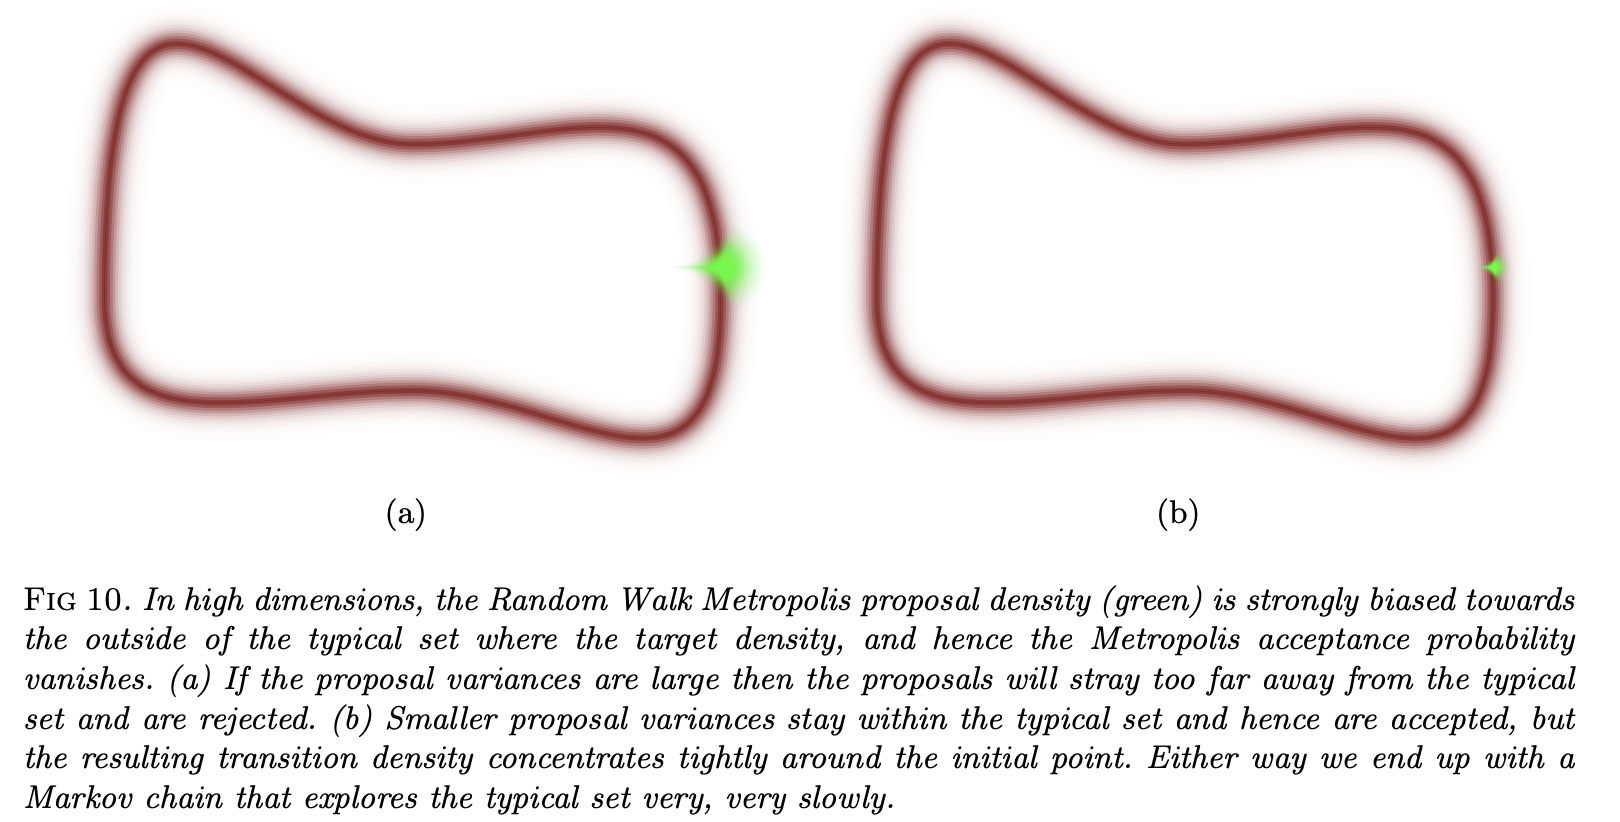
\includegraphics[scale = 0.5]{random_walk_high_dim.png}}
\end{minipage}
\caption{\footnotesize{\textbf{The challenge of random walk Metropolis-Hastings on high dimensional space.  \citep{betancourt2017conceptual}}}}
\label{fig: random_walk_high_dim}
\end{figure}

\item In order to make large jumps away from the initial point, and into new, unexplored regions of the typical set, we need to exploit information about the \underline{\textbf{\emph{geometry}}} of the \emph{typical set} itself. Specifically, we need transitions that can follow those \emph{\textbf{contours of high probability mass}}, coherently gliding through the typical set.

\item Hamiltonian Monte Carlo is the unique procedure for automatically generating this \emph{coherent exploration} for sufficiently well-behaved target distributions.
\end{itemize}

\begin{figure}
\begin{minipage}[t]{1\linewidth}
  \centering
  \centerline{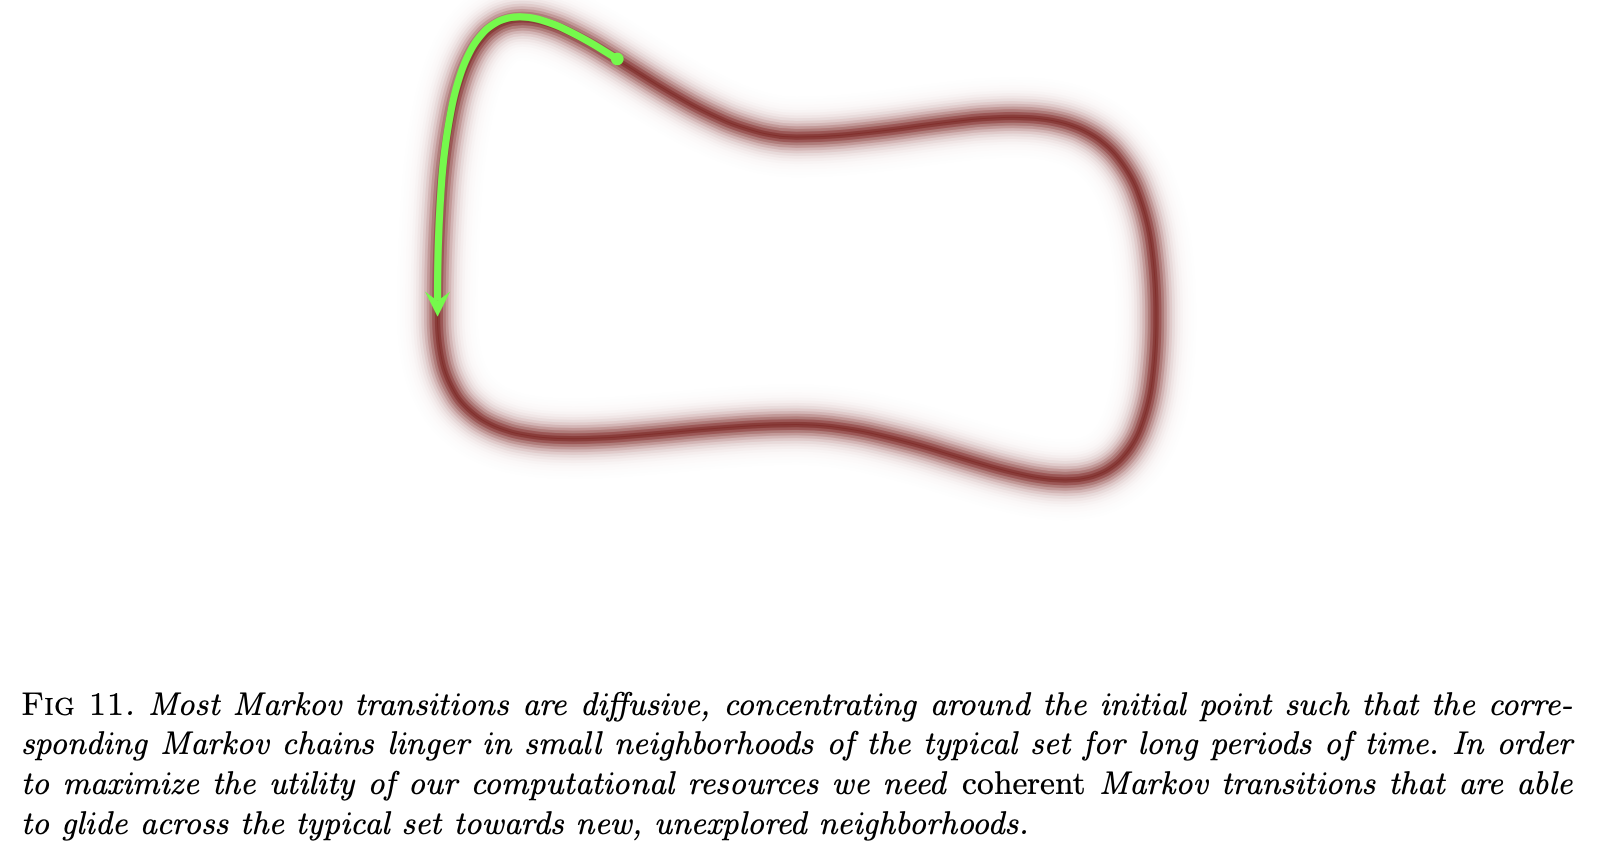
\includegraphics[scale = 0.5]{geometry_explore_typical_set.png}}
\end{minipage}
\caption{\footnotesize{\textbf{The Markov chain that is able to explore the contours of high probability mass is needed.}}}
\label{fig: geometry_explore_typical_set}
\end{figure}

\subsubsection{Hamiltonian Monte Carlo}
\begin{itemize}
\item Compare to MCMC, \underline{\emph{\textbf{Hamiltonian Monte Carlo (HMC)}}} \citep{brooks2011handbook} has some unique characteristics:
\begin{itemize}
\item HMC reply on the \underline{\textbf{\emph{Hamiltonian dynamic}}} to \textbf{explore} the parameter space. As oppose to the \emph{stochastic process} from MCMC, the HMC exploration process is \underline{\emph{\textbf{deterministic}}} based on the \emph{differential equations} \eqref{eqn: Hamilton_equation_1}, \eqref{eqn: Hamilton_equation_2}. HMC only need to simulate the \textbf{initial velocity/momentum} $\mb{v}(0)$ to start the Hamiltonian dynamic.

\item HMC \underline{\textbf{\emph{preserves the target distribution}}} $\pi$ by \emph{properties of Hamiltonian dynamic}, while the MCMC preserve the target distribution as the \emph{stationary distribution} of Markov chain.

\item Unlike the \emph{diffusion transition kernel} in MCMC, the transition process of HMC encodes \underline{\emph{\textbf{geometrical information}}} of the typical set via its associated \emph{\textbf{vector field}}. In other words, instead of fumbling around parameter space with random, uninformed jumps, we can follow the direction assigned to each at point for a small distance.  Continuing this process traces out a coherent trajectory through the typical set that efficiently moves us far away from the initial point to new, unexplored regions of the typical set \emph{as quickly as possible}.  

\item The performance of MCMC and its special case, Gibbs sampling, depend on a particular \emph{\textbf{parameterization}} of the target distribution. On the other hand, the design of Hamiltonian carefully remove the dependency on parameterization with additional geometric constraints while twisting the directions to align with the typical set. 

\item Compared to Random-walk Metropolis-Hastings, HMC reduces the correlation between successive sampled states by proposing moves to distant states which maintain a high probability of acceptance.
\end{itemize}

\begin{figure}
\begin{minipage}[t]{1\linewidth}
  \centering
  \centerline{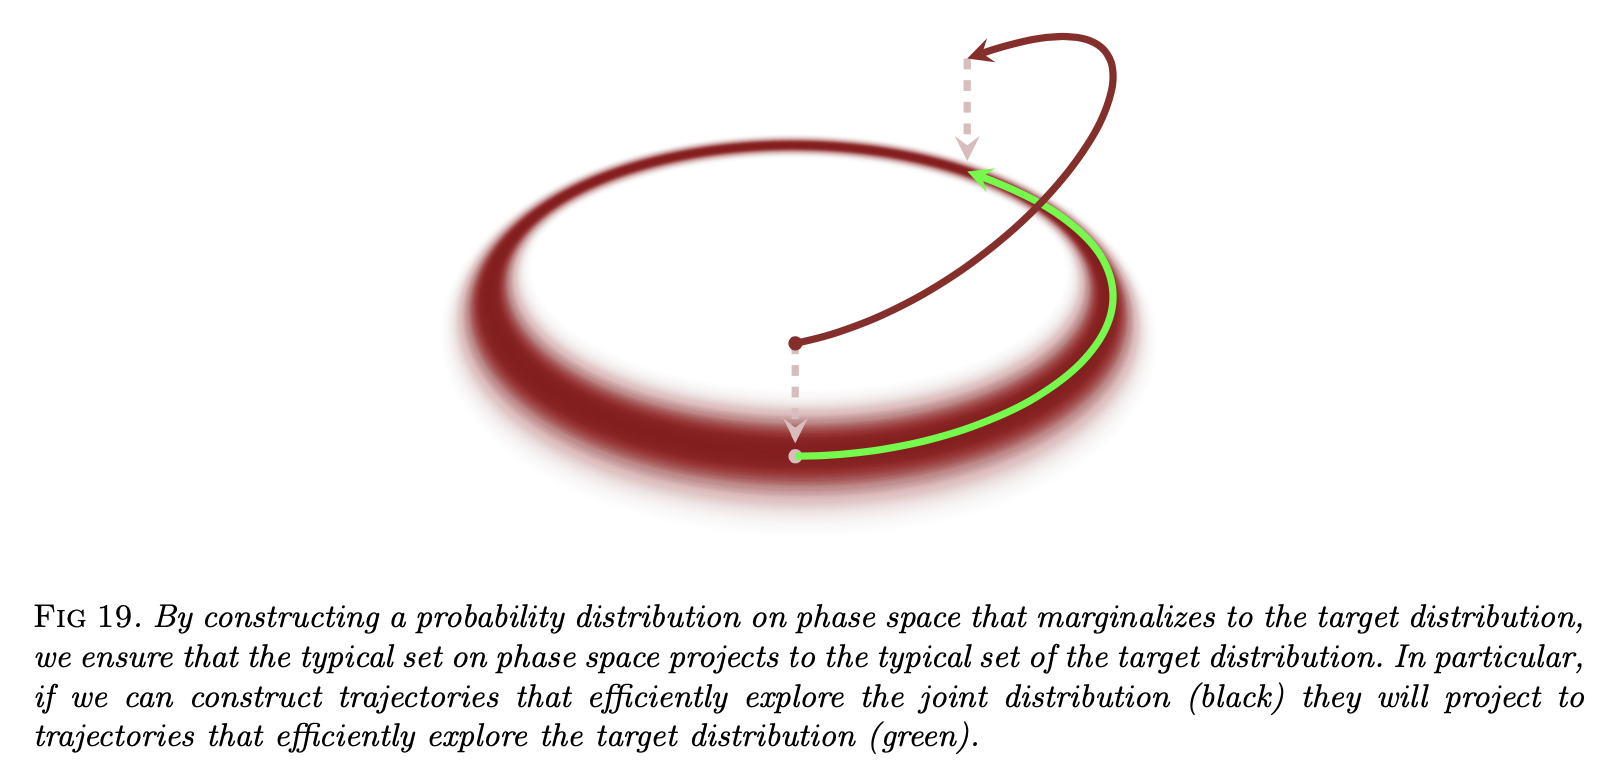
\includegraphics[scale = 0.5]{hmc_circle.png}}
\end{minipage}
\caption{\footnotesize{\textbf{By constructing a probability distribution on phase space that marginalizes to the target distribution, we ensure that the typical set on phase space projects to the typical set of the target distribution. \citep{betancourt2017conceptual}}}}
\label{fig: hmc_circle}
\end{figure}

\item Inspired by classical mechanic systems, the \underline{\textbf{key idea}} of \emph{\textbf{Hamiltonian Monte Carlo (HMC)}} is introduce \emph{\textbf{auxiliary momentum parameters}} in order to twist the gradient vector field into a vector field aligned with the typical set, and hence one capable of generating efficient exploration.

\item Consider the target distribution as
\begin{align}
\pi(\mb{x}, \mb{v}) &\propto \frac{1}{Z}\exp\paren{-\cH(\mb{x}, \mb{v})}, \label{eqn: hmc_target} 
\end{align} where $\mb{v}$ is the \emph{\textbf{auxiliary momentum parameters}}, $\mb{z} := (\mb{x}, \mb{v})$ is called \emph{\textbf{phase-space parameterization}}. The joint probability $\pi(\mb{x}, \mb{v})$ distribution on phase space is called the \emph{\textbf{canonical distribution}} or phase-space distribution.

\item Note that $\cH(\mb{x}, \mb{v})$ is \underline{\emph{\textbf{independent}}} of the details of any \emph{\textbf{parameterization}}, so does the \emph{canonical density} $\pi(\mb{x}, \mb{v})$ in \eqref{eqn: hmc_target}. Moreover, $\cH(\mb{x}, \mb{v})$ captures the \emph{\textbf{invariant probabilistic structure}} of the phase-space distribution and, most importantly, the \emph{\textbf{geometry}} of its typical set. 

\item We can factorize $\pi$ into
\begin{align}
\pi(\mb{x}, \mb{v}) &= \pi(\mb{v}|\mb{x})\pi(\mb{x}) \label{eqn: hmc_factorization} \\
-\log \pi(\mb{x}, \mb{v}) &= -\log \pi(\mb{v}|\mb{x}) - \log \pi(\mb{x}) \nonumber\\
&=\cK(\mb{x}, \mb{v}) + \cV(\mb{x}) := \cH(\mb{x}, \mb{v}).\label{eqn: hmc_factorization_2}
\end{align} where $\cK(\mb{x}, \mb{v})$ is the \emph{kinetic energy} and $ \cV(\mb{x})$ is the \emph{potential energy}. The potential energy is completely determined by the target distribution while \underline{the \emph{kinetic energy} is \emph{\textbf{unconstrained}}} and must be specified by the implementation.

This factorization guarantees that any trajectories exploring the typical set of the phase space distribution  $\pi(\mb{x}, \mb{v})$ will project to trajectories exploring the typical set of the target distribution $\pi(\mb{x})$.

\item Note that $\cH(\mb{x}, \mb{v})$ is \underline{\emph{\textbf{independent}}} of the details of any \emph{\textbf{parameterization}}, so does the \emph{canonical density} $\pi(\mb{x}, \mb{v})$ in \eqref{eqn: hmc_target}. Moreover, $\cH(\mb{x}, \mb{v})$ captures the \emph{\textbf{invariant probabilistic structure}} of the phase-space distribution and, most importantly, the \emph{\textbf{geometry}} of its typical set.

\item  Given \eqref{eqn: hmc_factorization_2}, recall from \eqref{eqn: Hamilton_dynamics_general} that
\begin{align}
\frac{d x^{i}}{dt} &=  \partdiff{\cK}{v_{i}} = -\partdiff{\log \pi(\mb{v}|\mb{x})}{v_{i}}, \quad  i=1,\ldots, d \nonumber\\
\frac{d v_{i}}{dt} &= - \partdiff{\cK}{x^{i}} - \partdiff{\cV}{x^{i}} = \partdiff{\log \pi(\mb{v}|\mb{x})}{x^{i}}+\partdiff{\log \pi(\mb{x})}{x^{i}}, \quad  i=1,\ldots, d \label{eqn: hmc_hamiltonian_eqn}
\end{align}
\end{itemize}


\subsection{Idealized Hamiltonian Monte Carlo}
\subsubsection{Formulation}
\begin{itemize}
\item Let $\phi_t : (\mb{x}, \mb{v}) \mapsto (\mb{x}_t(\mb{x}, \mb{v}), \mb{v}_t(\mb{x}, \mb{v}))$ be the trajectory characterized by differential equations \eqref{eqn: hmc_hamiltonian_eqn}. $\phi_t(\mb{x}, \mb{v})$ is the position and velocity/momentum at time $t$ starting from $(\mb{x}, \mb{v})$. 

\item The \underline{\emph{\textbf{idealized Hamiltonian Monte Carlo}}} \citep{betancourt2017conceptual, vishnoi2021introduction} is described as below:

\begin{enumerate}
\item For $t=1,2,\ldots, k$:
\begin{enumerate}
\item Given $\mb{X}_{t-1}$, generate a momentum $\mb{V}_{t-1}$ from conditional distribution $\pi(\mb{v}|\mb{X}_{t-1})$;
\item Set $(\mb{X}_{t}, \mb{V}_{t}) = \phi_{T}(\mb{X}_{t-1}, \mb{V}_{t-1})$ by integrating Hamilton’s equations for some time $T$
\end{enumerate}

\item Return $\mb{X}_{k}$ after projecting away the momentum.
\end{enumerate}
Composing these steps together yields a \emph{\textbf{Hamiltonian Markov transition}} composed of \emph{random trajectories} that rapidly explore the target distribution.

\item Using energy level set for Hamiltonian, 
\begin{align*}
\cH^{-1}(E) &= \set{(\mb{x}, \mb{v}): \cH(\mb{x}, \mb{v}) = E},
\end{align*} which are all $(2\,d - 1)$-dimensional, \emph{\textbf{compact}} surfaces in phase space. These \emph{\textbf{concentric level sets}} form a \emph{\textbf{foliation}}. The joint distribution $\pi(\mb{x}, \mb{v})$ thus can be decomposed via conditionals on energy level set:
\begin{align*}
\pi(\mb{x}, \mb{v}) &= \pi(\mb{\theta}_{E}\,|\,E)\pi(E),
\end{align*}.

\begin{figure}
\begin{minipage}[t]{1\linewidth}
  \centering
  \centerline{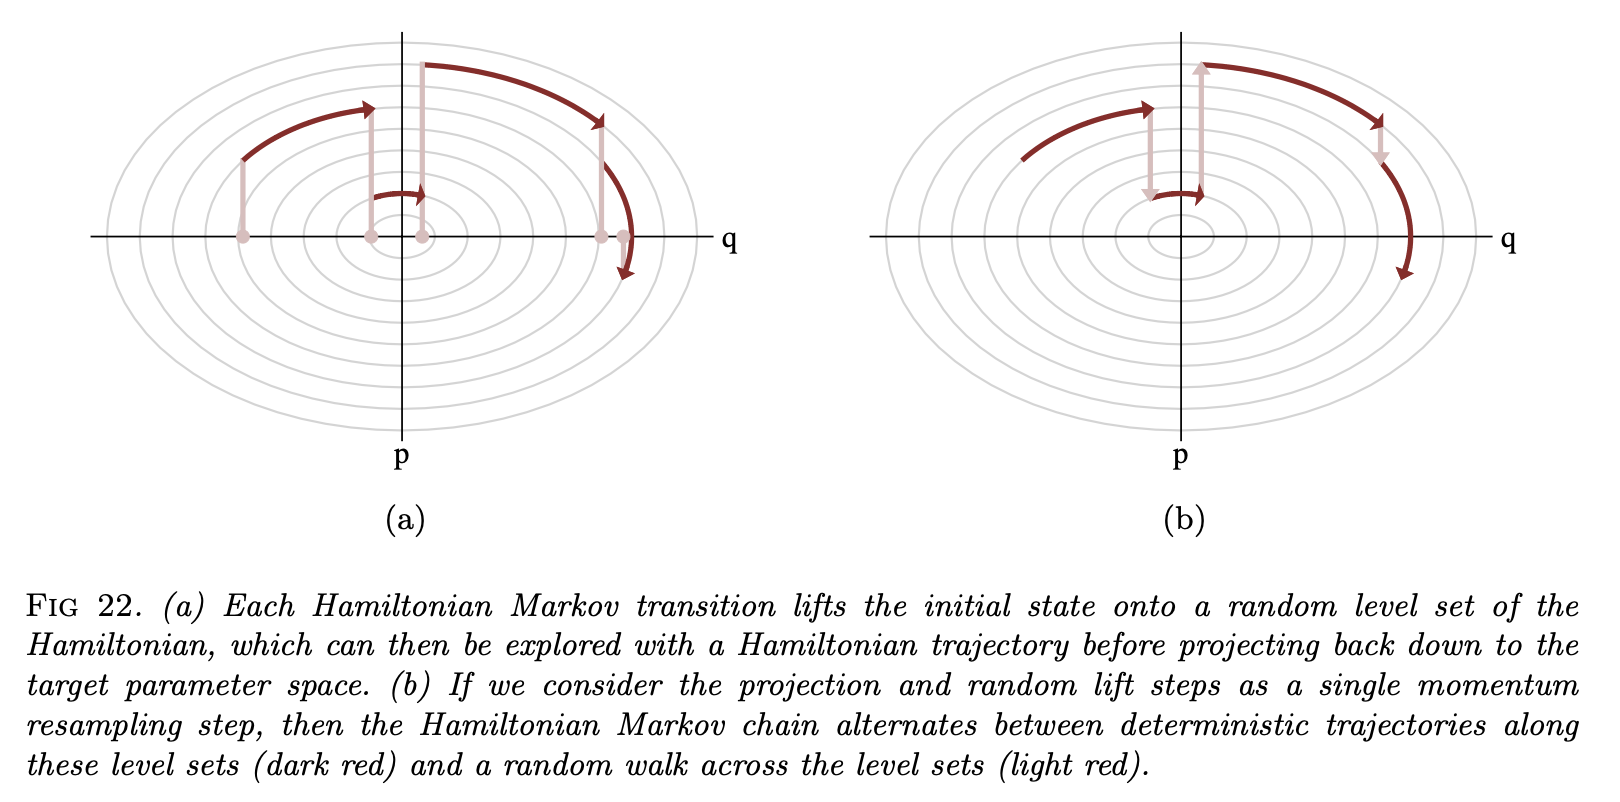
\includegraphics[scale = 0.5]{hmc_geomotry_process.png}}
\end{minipage}
\caption{\footnotesize{\textbf{Using level-sets, we see that HMC first explore within level set and then jump from one level set to another via random walk. \citep{betancourt2017conceptual}}}}
\label{fig: hmc_geomotry_process}
\end{figure}
\item We can see that the entire Hamiltonian Markov chain decouples into \textbf{\emph{two distinct phases}}: 
\begin{enumerate}
\item \emph{\textbf{deterministic}} exploration of individual \emph{level sets}
\item a \emph{\textbf{stochastic}} exploration \emph{\textbf{between}} the level sets themselves 
\end{enumerate}

\item  \begin{theorem} (\textbf{HMC Preserves the Target Density}) \citep{vishnoi2021introduction}
Suppose $(\mb{X}, \mb{V})$ is a sample from the density
\begin{align*}
\pi(\mb{x}, \mb{v}) &= \frac{1}{Z}\exp\paren{-\cH(\mb{x}, \mb{v})}d\mu(\mb{x}, \mb{v})
\end{align*} where $Z = \int \exp\paren{-\cH(\mb{x}, \mb{v})}d\mu(\mb{x}, \mb{v})$ is the partition function. Let $T > 0$ be the step size of the HMC. Then the density of $\phi_T(\mb{X}, \mb{V})$ is $\pi$ for any $T \ge 0$. Moreover the density of $\phi_T(\mb{X}_{t-1}, \mb{V}_{t-1})$, where $\mb{V}_{t-1} \sim \pi(\mb{v}|\mb{X}_{t-1})$ is also $\pi$. Thus, the \textbf{idealized HMC algorithms preserves} $\pi$.
\end{theorem}
\end{itemize}

\subsubsection{Euclidean-Gaussian Kinetic Energies}
\begin{itemize}
\item The first substantial \textbf{\emph{degree of freedom}} in the Hamiltonian Monte Carlo method that we can tune is the choice of the conditional probability distribution over the momentum or, equivalently, \textbf{the choice of a kinetic energy function}. Along with the target distribution, this choice completes the probabilistic structure on phase space which then determines the geometry of the microcanonical decomposition.

\item The simplest choice is to allow velocity/momentum $\mb{V}_{t}$ being \textbf{\emph{independent}} of $\mb{X}_{t}$, i.e. $\pi(\mb{v}|\mb{x}):= g(\mb{v})$. This is equivalent to assuming that \emph{the phase-space geometry} is \emph{\textbf{flat}}. The Hamiltonian Monte Carlo corresponds to a \emph{random-walk} across a foliation of the phase-space.

\item A natural choice of $g(\mb{v})$ is Normal distribution $\cN(\mb{v}\,|\, \mb{0}, \mb{\Sigma}_{v})$. Here, the covariance matrix $\mb{\Sigma}_{v}$ encodes an Euclidean metric in the phase-space. The corresponding kinetic energy is a \emph{\textbf{Euclidean-Gaussian kinetic energy}}
\begin{align}
\cK(\mb{v}) &= \frac{1}{2}\mb{v}^{T} \mb{\Sigma}_{v}^{-1} \mb{v} + \log \det{\mb{\Sigma}_{v}} + const.. \label{eqn: hmc_quatratic_kinetic}
\end{align}   And the Hamilton's equation is simplified as 
\begin{align}
\frac{d \mb{x}}{dt} &= \grad{\mb{v}}{\cK} = \mb{\Sigma}_{v}^{-1} \mb{v}  \nonumber\\
\frac{d \mb{v}}{dt} &= - \grad{\mb{x}}{\cV} = \grad{\mb{x}}{E} \label{eqn: hmc_hamiltonian_eqn_quar_k}
\end{align} where the target distribution $\pi(\mb{x}) \propto \exp(-E(\mb{x}))$.

\item Because the Euclidean structure over the momentum is dual to the Euclidean structure over the parameters, its interactions with the target distribution are straightforward to derive. Applying the transformation $\mb{p}' = \mb{\Sigma}_v^{-1/2}\mb{v}$ simplifies the kinetic energy, but remember that we have to apply the \emph{\textbf{opposite transformation}} to the parameters, $\mb{x}' = \mb{\Sigma}_v^{1/2}\mb{x}$, to preserve the Hamiltonian geometry.  Consequently, a choice of $\mb{\Sigma}_{v}^{-1}$ effectively \emph{\textbf{rotates}} and then \emph{\textbf{rescales}} the target \textbf{parameter} space, potentially \emph{\textbf{correlating}} or \textbf{\emph{de-correlating}} the target distribution and correspondingly \emph{\textbf{warping}} the energy level sets.

In particular, as the inverse Euclidean metric more closely resembles the covariance of the target distribution it de-correlates the target distribution, resulting in energy level sets that are more and more uniform and hence easier to explore. 
\end{itemize}

\subsection{Hamiltonian Monte Carlo in Practice}
\begin{itemize}
\item The \emph{\textbf{main obstruction}} to implementing the Hamiltonian Monte Carlo method is generating the Hamiltonian trajectories themselves. Aside from a few trivial examples, we \emph{cannot solve Hamilton’s equations exactly} and any implementation must instead solve them \emph{numerically}. \textbf{Numerical inaccuracies}, however, can quickly compromise the utility of even the most well-tuned Hamiltonian transition. 

\item Common ODE solvers suffer from an issue of \emph{\textbf{drift}}. As we numerically solve longer and longer trajectories the error in the solvers adds coherently, pushing the approximate trajectory away from the true trajectory and the typical set that we want to explore. Moreover, the magnitude of this drift rapidly increases with the dimension of phase space.

\item Fortunately, we can use the geometry of phase space itself to construct an extremely powerful family of numerical solvers, known as \underline{\emph{\textbf{symplectic integrators}}} \citep{liu2001monte, leimkuhler2004simulating,haier2006geometric,  betancourt2017conceptual, vishnoi2021introduction}, that are robust to phenomena like drift and enable high-performance implementations of the Hamiltonian Monte Carlo method.
\end{itemize}

\subsubsection{Symplectic Integrators}
\begin{itemize}
\item Symplectic integrators are powerful because the numerical trajectories they generate exactly \emph{\textbf{preserve phase space volume}}, just like the Hamiltonian trajectories they are approximating. Consequently, the numerical trajectories cannot drift away from the exact energy level set, instead oscillating near it even for long integration times.

\item For independent momentum distribution like the Euclidean-Gaussian kinetic energy, the symplectic integrator is called \emph{\textbf{leapfrog integrator}} \citep{brooks2011handbook}. 

\item The \underline{\emph{\textbf{Leapfrog Integrator}}} is described as below, where  $\epsilon$ is the time discretization, or step size:
\begin{enumerate}
\item Initialization: $\mb{x}_0 \leftarrow \mb{x}$, $\mb{v}_0 \leftarrow \mb{v}$.
\item For $0 \le t \le \lfloor \frac{T}{\epsilon}\rfloor$:
\begin{flalign*}
(a)\quad &\mb{v}_{t+\frac{1}{2}} \leftarrow \mb{v}_{t} - \frac{\epsilon}{2}\grad{\mb{x}}{\cV}(\mb{x}_{t})&\\
(b)\quad &\mb{x}_{t+1} \leftarrow \mb{x}_{t} + \epsilon\, \mb{\Sigma}_{v}^{-1}\mb{v}_{t+\frac{1}{2}}\\
(c)\quad &\mb{v}_{t+1} \leftarrow \mb{v}_{t+\frac{1}{2}} - \frac{\epsilon}{2}\grad{\mb{x}}{\cV}(\mb{x}_{t+1})
\end{flalign*}
\end{enumerate}

This simple but precise interleaving of discrete momentum and position updates ensures exact volume preservation on phase space, and hence the accurate numerical trajectories we need to realize the potential of a Hamiltonian transition.

\begin{figure}
\begin{minipage}[t]{1\linewidth}
  \centering
  \centerline{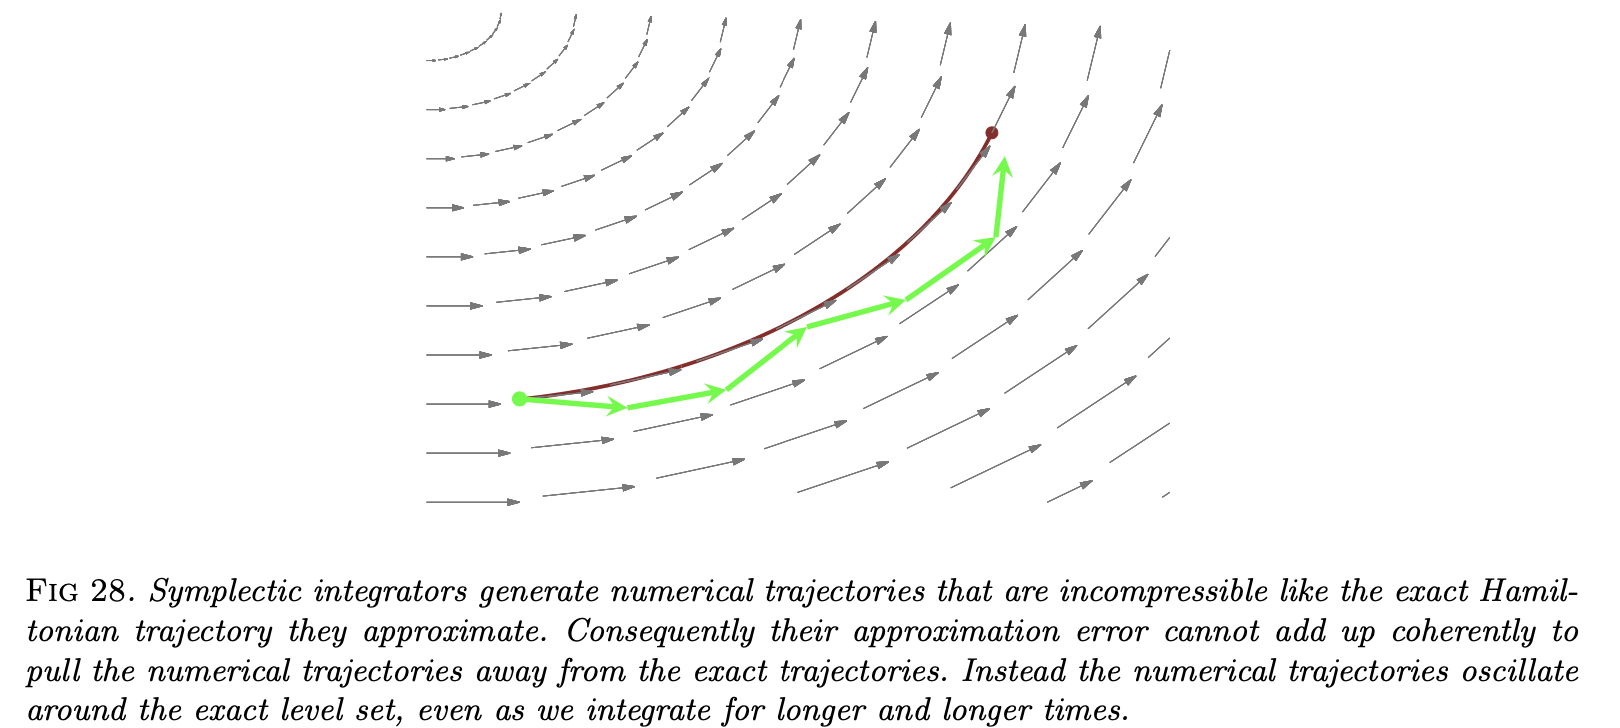
\includegraphics[scale = 0.5]{symplectic_integrator.png}}
\end{minipage}
\caption{\footnotesize{\textbf{Symplectic integrator will oscillate near exact level set even for long integration times. \citep{betancourt2017conceptual}}}}
\label{fig: symplectic_integrator}
\end{figure}

\item Employing symplectic integrators provides the opportunity to translate the theoretical performance of the Hamiltonian Monte Carlo method into a practical implementation. There remain, however, two obstructions to realizing this translation. 
\begin{itemize}
\item First, even though symplectic integrators are highly accurate, the small errors they do introduce will bias the resulting Hamiltonian transitions without an exact correction. 
\item Second, we have to be able to select a symplectic integrator well-suited to a given target distribution.
\end{itemize}
\end{itemize}

\subsubsection{Correcting for Symplectic Integrator Error}
\begin{itemize}
\item One particularly natural strategy for correcting the bias introduced by the error in a symplectic integrator is to treat the \emph{\textbf{Hamiltonian transition as the proposal}} for a Metropolis-Hastings scheme on phase space. 

\begin{figure}
\begin{minipage}[t]{1\linewidth}
  \centering
  \centerline{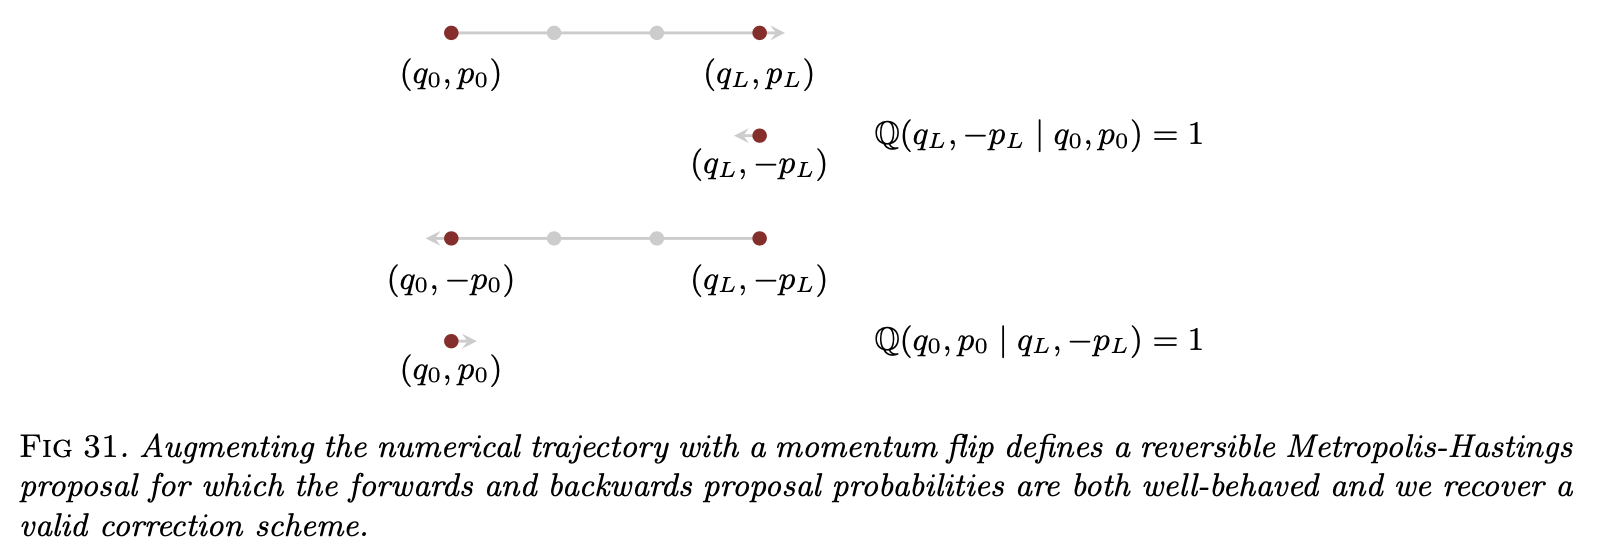
\includegraphics[scale = 0.6]{metro_hmc.png}}
\end{minipage}
\caption{\footnotesize{\textbf{Obtaining the reverse chain by flipping the sign of momentum. Note that the kinetic energy is symmetric to the change of sign in momentum. \citep{betancourt2017conceptual}}}}
\label{fig: metro_hmc}
\end{figure}

\item Suppose $(\mb{x}_{L}, \mb{v}_{L})$ be the last state of $L$ symplectic integrator steps starting from $(\mb{x}_{0}, \mb{v}_{0})$. \textbf{One issue} with computing the Metropolis-Hastings acceptance rate is that the transition kernel for HMC is determined by the symplectic integrator which can only move forward \emph{not backward}. In order to obtain the \emph{\textbf{reversible chain}}, we need to use the trick that \emph{\textbf{flipping the sign of momentum} will not change the kinetic energy}, thus not changing the overall distribution. Thus we will have the Hastings ratio computed as
\begin{align}
r(\mb{x}_{0}, \mb{v}_{0}; \mb{x}_{L}, -\mb{v}_{L}) &=\frac{\pi(\mb{x}_{L}, -\mb{v}_{L})\,K((\mb{x}_{L}, -\mb{v}_{L}); (\mb{x}_{0}, \mb{v}_{0}))}{\pi(\mb{x}_{0}, \mb{v}_{0})K((\mb{x}_{0}, \mb{v}_{0}); (\mb{x}_{L}, -\mb{v}_{L}))}  \nonumber\\
&=  \frac{\pi(\mb{x}_{L}, -\mb{v}_{L})}{\pi(\mb{x}_{0}, \mb{v}_{0})} \nonumber\\
&= \exp\paren{-\cH(\mb{x}_{L}, -\mb{v}_{L}) + \cH(\mb{x}_{0}, \mb{v}_{0})}\label{eqn: hmc_hastings_ratio}
\end{align}

\item Finally, we have \underline{\emph{\textbf{Metropolized Hamiltonian Monte Carlo}}} \citep{brooks2011handbook, betancourt2017conceptual}:
\begin{enumerate}
\item For $t=1,2,\ldots, k$:
\begin{enumerate}
\item Generate a momentum $\mb{V}_{t-1}$ from Normal distribution $\cN(\mb{0}, \mb{\Sigma}_{v})$;
\item Set $(\mb{X}', \mb{V}') = \widehat{\phi}_{T}(\mb{X}_{t-1}, \mb{V}_{t-1})$ as the last state of $T$ symplectic integrator steps starting from 
$(\mb{X}_{t-1}, \mb{V}_{t-1})$. 

\item Compute the Hastings ratio:
\begin{align*}
r(\mb{X}_{t-1}, \mb{V}_{t-1}; \mb{X}', -\mb{V}') &= \exp\paren{-\cH(\mb{X}', -\mb{V}') + \cH(\mb{X}_{t-1}, \mb{V}_{t-1})}
\end{align*}

\item Accept $\mb{X}_{t} = \mb{X}'$ with probability 
\begin{align*}
\alpha(\mb{X}_{t-1}, \mb{V}_{t-1}; \mb{X}', -\mb{V}') &= \min\set{1,\;r(\mb{X}_{t-1}, \mb{V}_{t-1}; \mb{X}', -\mb{V}')}
\end{align*}

\item Otherwise, accept $\mb{X}_{t} = \mb{X}_{t-1}$.
\end{enumerate}
\end{enumerate}

\item Symplectic integrators are not exactly energy preserving, causing their numerical trajectories to deviate from the target energy level set. In particular, sampling a state uniformly from any numerical trajectory will not generate a sample from the canonical distribution. This error, however, can be exactly corrected by sampling from the trajectory not uniformly but rather with weights proportional to the desired canonical density function \citep{betancourt2017conceptual}.

\item Regarding the \emph{\textbf{robustness}} of the HMC, preliminary results show that even simple implementations of the Hamiltonian Monte Carlo method are geometrically ergodic over a large class of target distributions, larger than the class for non-gradient based algorithms like Random-walk Metropolis-Hastings.

\item There also some concerns in practice:
\begin{itemize}
\item In practice, \emph{\textbf{longer trajectory}} $T$ is preferred so that the end state is less correlated with the initial state. However, it will have larger cost of simulation time.

\item Also, if the \emph{\textbf{kinetic energy}} is \emph{poorly-chosen} then the marginal energy distribution can become heavy-tailed itself in which case the stochastic exploration between level sets will become so slow that after any finite number of transitions the exploration of the Markov chain will be incomplete.

\item Another common obstruction to geometric ergodicity is neighborhoods in parameter space where the target distribution exhibits \emph{\textbf{large curvature}}. Most Markov transitions are not able to resolve these narrow neighborhoods, resulting in incomplete exploration and biased Markov chain Monte Carlo estimators. 

\item Finally, HMC requires computation on the \emph{\textbf{gradients}} in the symplectic integrator. It would be computational expensive if the target distribution has complex form.
\end{itemize}
\end{itemize}


\section{Monte Carlo Optimization}
\begin{itemize}
\item Similar to the problem of integration, differences between the numerical approach and the simulation approach to the problem
\begin{align}
\max_{\mb{x}\in \cX} h(\mb{x}) \label{eqn: stochastic_opt}
\end{align} lie in the treatment of the function $h$. 
\begin{itemize}
\item In approaching an optimization problem using deterministic numerical methods, the \emph{\textbf{analytical properties}} of the target function (\emph{convexity}, \emph{boundedness}, \emph{smoothness}) are often paramount.
\item For the simulation approach, we are more concerned with $h$ from a \emph{\textbf{probabilistic}} (rather than analytical) point of view. 
\end{itemize}

\item We want to distinguish between two approaches to \underline{\emph{\textbf{Monte Carlo optimization}}} \citep{robert1999monte}.
\begin{itemize}
\item  The first is an \underline{\emph{\textbf{exploratory approach}}}, in which the goal is to optimize the function $h$ by \emph{describing its entire range}. The \emph{actual properties} of the function play a \emph{lesser role} here, with the Monte Carlo aspect more closely tied to the \emph{\textbf{exploration of the entire space}} $\cX$, even though, for instance, the slope of $h$ can be used to speed up the exploration.

\item The second approach is based on a \underline{\emph{\textbf{probabilistic approximation}}} of the \emph{objective function} $h$ and is somewhat of a \emph{preliminary step} to the actual optimization. Here, the Monte Carlo aspect \emph{\textbf{exploits the probabilistic properties of the function}} $h$ to come up with an acceptable approximation and is less concerned with exploring $\cX$. For instance, \emph{Missing data methods}, such as the \emph{EM algorithm}, are closely related to tied to this idea.
\end{itemize}

\end{itemize}
\subsection{Gradient Methods}
\begin{itemize}
\item The gradient method is a \emph{deterministic} numerical approach to the problem \eqref{eqn: stochastic_opt}. It produces a sequence $(\mb{x}_{t})$ that converges to the exact solution of \eqref{eqn: stochastic_opt}, $\mb{x}^{*}$, when the domain $\cX \subseteq \bR^d$ and the function $(-h)$ are both \emph{convex}. The sequence $(\mb{x}_{t})$ is constructed in a \emph{\textbf{recursive}} manner through
\begin{align*}
\mb{x}_{t+1} &= \mb{x}_{t} + \alpha_{t}\grad{}{h(\mb{x}_t)}, \quad \alpha_t > 0.
\end{align*}

\item In more general setups (that is, when the function or the space is less regular), equation above can be modified by stochastic perturbations to again achieve convergence. One of these stochastic modifications is to choose a second sequence $(\beta_t)$ to define the chain  $(\mb{x}_{t})$ by
\begin{align}
\mb{x}_{t+1} &= \mb{x}_{t} + \frac{\alpha_{t}}{2\beta_{t}}\Delta\,h(\mb{x}_t, \beta_{t}\mb{\xi}_{t})\mb{\xi}_{t}, \quad \alpha_t > 0. \label{eqn: sgd}\\
\text{where }\Delta\,h(\mb{x}_t, \beta_{t}\mb{\xi}_{t}) &= \paren{h(\mb{x}_t + \beta_{t}\mb{\xi}_{t}) - h(\mb{x}_t - \beta_{t}\mb{\xi}_{t})} \approx 2\,\beta_{t}\norm{\mb{\xi}_{t}}{2}\grad{}{h(\mb{x}_t)}, \nonumber
\end{align} and the variables $\mb{\xi}_{t}$ are uniformly distributed on the unit sphere $\norm{\mb{\xi}_{t}}{2} = 1$.

In contrast to the deterministic approach, this method does not necessarily proceed along the \emph{steepest slope} in $(\mb{x}_{t})$, but this property is sometimes a \emph{plus} in the sense that it may \emph{avoid being trapped in \textbf{local maxima}} or in \emph{\textbf{saddlepoints}} of $h$.

\item Consider the objective function is the sample average of log-likelihood function 
$h(\mb{\theta}): = \sum_{i=1}^{N}\ell(\mb{\theta}; \mb{x}_i)$. The \emph{\textbf{stochastic gradient ascent}} is of form
\begin{align}
\mb{\theta}_{t+1} &= \mb{\theta}_{t} + \alpha_{t}\grad{\mb{\theta}}{\ell(\mb{\theta}_{t}; \mb{\xi}_t)}, \quad \alpha_t > 0.
\label{eqn: sgd_2}
\end{align} where $\mb{\xi}_{t} \sim \set{\mb{x}_1, \ldots, \mb{x}_{n}}$ is a random sample from data.
\end{itemize}
\subsection{Simulated Annealing}
\begin{itemize}
\item The \emph{\textbf{fundamental idea}} of \emph{\textbf{simulated annealing methods}} is that a change of scale, called \emph{\textbf{temperature}}, allows for faster moves on the surface of the function $h$ to maximize, whose negative is called \emph{\textbf{energy}}. Therefore, rescaling partially avoids the trapping attraction of local maxima.

\item Given a temperature parameter $T > 0$, a sample $(\mb{x}_{t})_t$. is generated from the distribution
\begin{align}
\pi(\mb{x}) &\propto \exp\paren{\frac{h(\mb{x})}{T}}
\end{align} As $T$ decreases toward $0$, the values simulated from this distribution become concentrated in a narrower and narrower neighborhood of the \emph{local maxima} of $h$

\item In Simulated Annealing, we run a fixed number of $N_k$ iterations of MCMC (\emph{Metropolis-Hastings} or \emph{Gibbs sampling}) so that $(\mb{X}^{(k)}_t)$ follows the stationary distribution $\pi_k(\mb{x}) \propto \exp(h(\mb{x})/T_{k})$. Then we decrease temperature $T_{k}$ to $T_{k+1}$ and restart the MCMC with last update $\mb{X}_{k}$. As $T_{k}\rightarrow 0$, the target distribution is approaching to an indicator on its mode, thus the simulated samples would be close to the optimal solution.

%\item Simulated annealing is essentially using MCMC to generate simulated samples from $\pi_k(\mb{x}) \propto \exp(h(\mb{x})/T_{k})$
%\item Simulated annealing is essentially a Random-walk Metropolis-Hastings algorithm, with a new proposal being accepted with probability $\min\set{1, \exp(\Delta h_t/T)}$ where $\Delta h_t = h(\mb{\xi}) - h(\mb{x}_t)$. Depending on the temperature $T$, there is non-zero probability of accepting a new proposal even if it is not local maximal. This property allows the algorithm to escape the attraction of $\mb{x}_t$ if $\mb{x}_t$ is a local maximum of $h$.

\item The \underline{\emph{\textbf{Simulated Annealing algorithm}}} can be implemented as 
\begin{enumerate}
\item Simulate $\mb{\xi}$ from an \emph{instrumental distribution} with density $g(\norm{\mb{\xi} - \mb{X}_{t}}{})$;
\item Accept $\mb{X}_{t+1} = \mb{\xi}$ with probability
\begin{align*}
\alpha(\mb{X}_t, \mb{\xi})&= \min\set{1, \exp\paren{\frac{\Delta h_{t}}{T_{t}}}}
\end{align*} where $\Delta h_t := h(\mb{\xi}) - h(\mb{X}_t)$;
\item Otherwise, accept $\mb{X}_{t+1} = \mb{X}_t$.
\item Update $T_{t}$ to $T_{t+1}$.
\end{enumerate}

\item  Since there is non-zero probability of accepting a new proposal even if it is not local maximal, it allows the algorithm to \emph{escape the attraction} of $\mb{x}_t$ if $\mb{x}_t$ is a local maximum of $h$. The temperature $T_{k}$ controls the probability of acceptance of non-optimal proposal.
\end{itemize}

\subsection{Simulated Tempering}
\begin{itemize}
\item \emph{\textbf{Simulated Tempering (ST)}} is proposed to let a MCMC scheme move more freely in the state space \citep{liu2001monte}.

\item Define a new target distribution, $\pi(\mb{x}, i) \propto c_{i}\exp\set{-h(\mb{x})/T_{i}}$ on the augmented space $(\mb{x}, i) \in \cX \times I$. Here, the $c_i$ are constants that can be controlled by the user and they should be tuned so that each tempered distribution in the system should have a roughly equal chance to be visited. Ideally, the $c_i$ should be proportional to the reciprocal of the $i$-th partition function, $Z_i = \int \exp\set{-h(\mb{x})/T_i}$.

\item The \underline{\emph{\textbf{Simulated Tempering (ST)}}} is described as 
\begin{enumerate}
\item With the current state $(\mb{X}_{t},\, i_{t}) = (\mb{x}, \,i)$, we draw $u\sim \cU[0,1]$.
\item (\emph{\textbf{Update sample}}) If $u \le \alpha_0$, we let $i_{t+l} = i$ and let $\mb{X}_{t+1}$ be drawn from a \emph{\textbf{MCMC transition}} $K_i(\mb{x}, \mb{x}_{t+1})$ that leaves $\pi_i\propto \exp(h(\mb{x})/T_{i})$ invariant.

\item (\emph{\textbf{Update temperature}}) If $u > \alpha_0$, we let $\mb{X}_{t+l} = \mb{x}$ and propose a \emph{\textbf{level transition}}, $i \rightarrow i'$, from a transition function $\alpha(i, i')$ (usually a nearest-neighbor simple random walk with reflecting boundary), and let $i_{t+1} = i'$ with probability
\begin{align*}
\min\set{1, \frac{c_{i'}\,\pi_{i'}(\mb{x})\,\alpha(i', i) }{ c_{i}\,\pi_i(\mb{x})\,\alpha(i, i')}};
\end{align*} otherwise accept $i_{t+1} = i$.
\end{enumerate} 
\end{itemize}

\subsection{Monte Carlo EM}
\begin{itemize}
\item Given observation $y$ and latent variables $\mb{x}$, the objective function for missing data problem is the \emph{incomplete likelihood}
\begin{align*}
\ell(\mb{\theta}|\mb{y}) &= \E{}{\ell_{c}(\mb{\theta}|\mb{y}, \mb{X})} = \int_{\cX}\ell_{c}(\mb{\theta}|\mb{x}, \mb{y})d\mb{x}
\end{align*} We refer to the function $\ell_{c}(\mb{\theta}|\mb{x}, \mb{y}) = p(\mb{x}, \mb{y} | \mb{\theta})$ as the \emph{complete-data likelihood}, which corresponds to the observation of the complete data $(\mb{x}, \mb{y})$ and $g(\mb{y}|\mb{\theta}) = \ell(\mb{\theta}|\mb{y}) $ is marginal distribution.

\item We can obtain lower bound of incomplete log-likelihood by introducing the conditional distribution $q(\mb{x}|\mb{y},\mb{\theta}):= \frac{p(\mb{x}, \mb{y} | \mb{\theta})}{g(\mb{x}| \mb{\theta})}$:
\begin{align*}
\log\ell(\mb{\theta}|\mb{y})  = \log \int_{\cX}p(\mb{x}, \mb{y} | \mb{\theta})d\mb{x} 
&= \log \int_{\cX} q(\mb{x}|\mb{y},\mb{\theta}) \frac{p(\mb{x}, \mb{y} | \mb{\theta})}{q(\mb{x}|\mb{y},\mb{\theta})}  d\mb{x} \\
&\ge \int_{\cX}q(\mb{x}|\mb{y},\mb{\theta})\log\frac{p(\mb{x}, \mb{y} | \mb{\theta})}{q(\mb{x}|\mb{y},\mb{\theta})}  d\mb{x}  \\
&= \E{q}{\ell_{c}(\mb{\theta}|\mb{x}, \mb{y})} - \E{q}{q(\mb{x}|\mb{y},\mb{\theta})}.
\end{align*} Denote the expected log-likelihood by
\begin{align*}
Q(\mb{\theta}|\mb{\theta}_{0}, \mb{y}) &:= \E{\mb{\theta}_{0}}{\ell_{c}(\mb{\theta}|\mb{x}, \mb{y})} 
\end{align*} 

\item The \emph{\textbf{EM (Expectation-Maximization) algorithm}} consists of two steps iteratively:
\begin{enumerate}
\item (\textbf{E-Step}): Compute $Q(\mb{\theta}|\mb{\theta}_{t}, \mb{y}) = \E{\mb{\theta}_{t}}{\ell_{c}(\mb{\theta}|\mb{x}, \mb{y})} $ with respect to $q(\mb{x}|\mb{y},\mb{\theta}_t)$
\item (\textbf{M-Step}): Maximize parameter $\mb{\theta}_{t+1} = \arg\max_{\mb{\theta}}Q(\mb{\theta}|\mb{\theta}_{t}, \mb{y})$
\end{enumerate}

\item It can be shown that EM algorithm increase the incomplete log-likelihood at each iteration:
\begin{align*}
\log\ell(\mb{\theta}_{t}|\mb{y}) \ge \log\ell(\mb{\theta}_{t-1}|\mb{y})
\end{align*}

\item A difficulty with the implementation of the EM algorithm is that each "E-step" requires the computation of the expected log likelihood $Q(\mb{\theta}|\mb{\theta}_{0}, \mb{y})$. An alternative solution is to approximate the expectation via Monte Carlo simulation, i.e. 
\begin{align}
\widehat{Q}_{m}(\mb{\theta}|\mb{\theta}_{0}, \mb{y}) &= \frac{1}{m}\sum_{t=1}^{m}\ell_{c}(\mb{\theta}|\mb{X}_i, \mb{y}_i)
\end{align} where samples of missing data $\mb{X}_i \sim q(\mb{x}|\mb{y}_{i},\mb{\theta}_0), i=1,\ldots, m$.

\item As $m\rightarrow \infty$, $\widehat{Q}_{m}(\mb{\theta}|\mb{\theta}_{0}, \mb{y}) \rightarrow Q(\mb{\theta}|\mb{\theta}_{0}, \mb{y})$.

\begin{figure}
\begin{minipage}[t]{1\linewidth}
  \centering
  \centerline{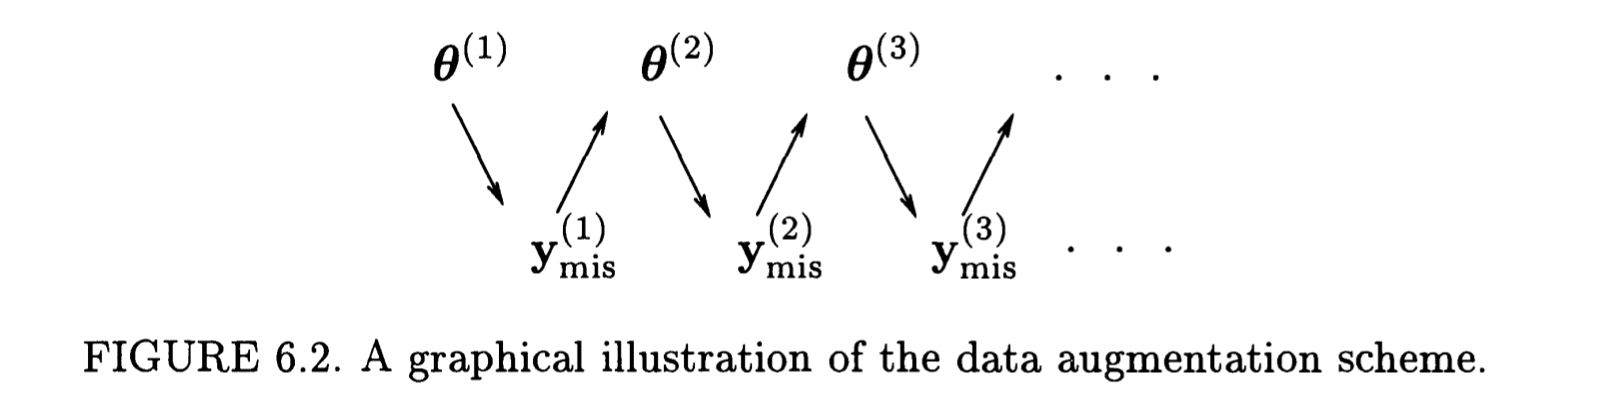
\includegraphics[scale = 0.5]{data_augmentation.png}}
\end{minipage}
\caption{\footnotesize{\textbf{Scheme for iteratively fill in missing data and update parameter \citep{liu2001monte}}}}
\label{fig: data_augmentation}
\end{figure}
\end{itemize}
\newpage
\bibliographystyle{plainnat}
\bibliography{book_reference.bib}
\end{document}